\documentclass[]{article}
\usepackage{lmodern}
\usepackage{amssymb,amsmath}
\usepackage{ifxetex,ifluatex}
\usepackage{fixltx2e} % provides \textsubscript
\ifnum 0\ifxetex 1\fi\ifluatex 1\fi=0 % if pdftex
  \usepackage[T1]{fontenc}
  \usepackage[utf8]{inputenc}
\else % if luatex or xelatex
  \ifxetex
    \usepackage{mathspec}
  \else
    \usepackage{fontspec}
  \fi
  \defaultfontfeatures{Ligatures=TeX,Scale=MatchLowercase}
\fi
% use upquote if available, for straight quotes in verbatim environments
\IfFileExists{upquote.sty}{\usepackage{upquote}}{}
% use microtype if available
\IfFileExists{microtype.sty}{%
\usepackage{microtype}
\UseMicrotypeSet[protrusion]{basicmath} % disable protrusion for tt fonts
}{}
\usepackage[margin=1in]{geometry}
\usepackage{hyperref}
\hypersetup{unicode=true,
            pdftitle={A Tutorial on Hidden Markov Models using Stan},
            pdfauthor={Luis Damiano (Universidad Nacional de Rosario), Brian Peterson (University of Washington), Michael Weylandt (Rice University)},
            pdfborder={0 0 0},
            breaklinks=true}
\urlstyle{same}  % don't use monospace font for urls
\usepackage{color}
\usepackage{fancyvrb}
\newcommand{\VerbBar}{|}
\newcommand{\VERB}{\Verb[commandchars=\\\{\}]}
\DefineVerbatimEnvironment{Highlighting}{Verbatim}{commandchars=\\\{\}}
% Add ',fontsize=\small' for more characters per line
\usepackage{framed}
\definecolor{shadecolor}{RGB}{248,248,248}
\newenvironment{Shaded}{\begin{snugshade}}{\end{snugshade}}
\newcommand{\KeywordTok}[1]{\textcolor[rgb]{0.13,0.29,0.53}{\textbf{{#1}}}}
\newcommand{\DataTypeTok}[1]{\textcolor[rgb]{0.13,0.29,0.53}{{#1}}}
\newcommand{\DecValTok}[1]{\textcolor[rgb]{0.00,0.00,0.81}{{#1}}}
\newcommand{\BaseNTok}[1]{\textcolor[rgb]{0.00,0.00,0.81}{{#1}}}
\newcommand{\FloatTok}[1]{\textcolor[rgb]{0.00,0.00,0.81}{{#1}}}
\newcommand{\ConstantTok}[1]{\textcolor[rgb]{0.00,0.00,0.00}{{#1}}}
\newcommand{\CharTok}[1]{\textcolor[rgb]{0.31,0.60,0.02}{{#1}}}
\newcommand{\SpecialCharTok}[1]{\textcolor[rgb]{0.00,0.00,0.00}{{#1}}}
\newcommand{\StringTok}[1]{\textcolor[rgb]{0.31,0.60,0.02}{{#1}}}
\newcommand{\VerbatimStringTok}[1]{\textcolor[rgb]{0.31,0.60,0.02}{{#1}}}
\newcommand{\SpecialStringTok}[1]{\textcolor[rgb]{0.31,0.60,0.02}{{#1}}}
\newcommand{\ImportTok}[1]{{#1}}
\newcommand{\CommentTok}[1]{\textcolor[rgb]{0.56,0.35,0.01}{\textit{{#1}}}}
\newcommand{\DocumentationTok}[1]{\textcolor[rgb]{0.56,0.35,0.01}{\textbf{\textit{{#1}}}}}
\newcommand{\AnnotationTok}[1]{\textcolor[rgb]{0.56,0.35,0.01}{\textbf{\textit{{#1}}}}}
\newcommand{\CommentVarTok}[1]{\textcolor[rgb]{0.56,0.35,0.01}{\textbf{\textit{{#1}}}}}
\newcommand{\OtherTok}[1]{\textcolor[rgb]{0.56,0.35,0.01}{{#1}}}
\newcommand{\FunctionTok}[1]{\textcolor[rgb]{0.00,0.00,0.00}{{#1}}}
\newcommand{\VariableTok}[1]{\textcolor[rgb]{0.00,0.00,0.00}{{#1}}}
\newcommand{\ControlFlowTok}[1]{\textcolor[rgb]{0.13,0.29,0.53}{\textbf{{#1}}}}
\newcommand{\OperatorTok}[1]{\textcolor[rgb]{0.81,0.36,0.00}{\textbf{{#1}}}}
\newcommand{\BuiltInTok}[1]{{#1}}
\newcommand{\ExtensionTok}[1]{{#1}}
\newcommand{\PreprocessorTok}[1]{\textcolor[rgb]{0.56,0.35,0.01}{\textit{{#1}}}}
\newcommand{\AttributeTok}[1]{\textcolor[rgb]{0.77,0.63,0.00}{{#1}}}
\newcommand{\RegionMarkerTok}[1]{{#1}}
\newcommand{\InformationTok}[1]{\textcolor[rgb]{0.56,0.35,0.01}{\textbf{\textit{{#1}}}}}
\newcommand{\WarningTok}[1]{\textcolor[rgb]{0.56,0.35,0.01}{\textbf{\textit{{#1}}}}}
\newcommand{\AlertTok}[1]{\textcolor[rgb]{0.94,0.16,0.16}{{#1}}}
\newcommand{\ErrorTok}[1]{\textcolor[rgb]{0.64,0.00,0.00}{\textbf{{#1}}}}
\newcommand{\NormalTok}[1]{{#1}}
\usepackage{longtable,booktabs}
\usepackage{graphicx,grffile}
\makeatletter
\def\maxwidth{\ifdim\Gin@nat@width>\linewidth\linewidth\else\Gin@nat@width\fi}
\def\maxheight{\ifdim\Gin@nat@height>\textheight\textheight\else\Gin@nat@height\fi}
\makeatother
% Scale images if necessary, so that they will not overflow the page
% margins by default, and it is still possible to overwrite the defaults
% using explicit options in \includegraphics[width, height, ...]{}
\setkeys{Gin}{width=\maxwidth,height=\maxheight,keepaspectratio}
\IfFileExists{parskip.sty}{%
\usepackage{parskip}
}{% else
\setlength{\parindent}{0pt}
\setlength{\parskip}{6pt plus 2pt minus 1pt}
}
\setlength{\emergencystretch}{3em}  % prevent overfull lines
\providecommand{\tightlist}{%
  \setlength{\itemsep}{0pt}\setlength{\parskip}{0pt}}
\setcounter{secnumdepth}{5}
% Redefines (sub)paragraphs to behave more like sections
\ifx\paragraph\undefined\else
\let\oldparagraph\paragraph
\renewcommand{\paragraph}[1]{\oldparagraph{#1}\mbox{}}
\fi
\ifx\subparagraph\undefined\else
\let\oldsubparagraph\subparagraph
\renewcommand{\subparagraph}[1]{\oldsubparagraph{#1}\mbox{}}
\fi

%%% Use protect on footnotes to avoid problems with footnotes in titles
\let\rmarkdownfootnote\footnote%
\def\footnote{\protect\rmarkdownfootnote}

%%% Change title format to be more compact
\usepackage{titling}

% Create subtitle command for use in maketitle
\newcommand{\subtitle}[1]{
  \posttitle{
    \begin{center}\large#1\end{center}
    }
}

\setlength{\droptitle}{-2em}
  \title{A Tutorial on Hidden Markov Models using Stan}
  \pretitle{\vspace{\droptitle}\centering\huge}
  \posttitle{\par}
  \author{Luis Damiano (Universidad Nacional de Rosario), Brian Peterson
(University of Washington), Michael Weylandt (Rice University)}
  \preauthor{\centering\large\emph}
  \postauthor{\par}
  \predate{\centering\large\emph}
  \postdate{\par}
  \date{2017-12-15}

\usepackage{amsmath}
\usepackage{hyperref} % links
\usepackage{booktabs}

% Math operators
\newcommand{\argmax}{\arg\!\max}
\newcommand{\argmin}{\arg\!\min}
\newcommand\ev[1]{E\left\langle#1\right\rangle}
\newcommand\vv[1]{V\left\langle#1\right\rangle}

% Math commands
\newcommand{\mat}[1]{\mathbf{#1}}

% Math symbols
\newcommand{\NN}{\mathcal{N}}
\newcommand{\UU}{\mathcal{U}}
\newcommand{\LL}{\mathcal{L}}
\newcommand{\RR}{\mathbb{R}}

% Links and colours
\hypersetup{hidelinks} % no box around links
\hypersetup{ % links with pretty colours
  colorlinks   = true, % Colours links instead of ugly boxes
  urlcolor     = blue, % Colour for external hyperlinks
  linkcolor    = blue, % Colour of internal links
  citecolor   = red % Colour of citations
}

\begin{document}
\maketitle

{
\setcounter{tocdepth}{2}
\tableofcontents
}
This case study documents the implementation in
\href{http://mc-stan.org/}{Stan} (Carpenter et al. 2016) of the Hidden
Markov Model (HMM) for unsupervised learning (Baum and Petrie 1966; Baum
and Eagon 1967; Baum and Sell 1968; Baum et al. 1970; Baum 1972).
Additionally, we present the adaptations needed for the Input-Output
Hidden Markov Model (IOHMM). IOHMM is an architecture proposed by Bengio
and Frasconi (1995) to map input sequences, sometimes called the control
signal, to output sequences. Compared to HMM, it aims at being
especially effective at learning long term memory, that is when
input-output sequences span long points. In all cases, we provide a
fully Bayesian estimation of the model parameters and inference on
hidden quantities, namely filtered state belief, smoothed state belief
and jointly most probable state path.

\emph{A Tutorial on Hidden Markov Models using Stan} is licensed under
CC-BY 4.0. See the \href{LICENSE.md}{LICENSE} file for details. All
files are available in the
\href{https://github.com/luisdamiano/stancon18}{stancon18} GitHub
repository.

\begin{center}\rule{0.5\linewidth}{\linethickness}\end{center}

\section{The Hidden Markov Model}\label{the-hidden-markov-model}

Real-world processes produce observable outputs characterized as
signals. These can be discrete or continuous in nature, be pure or
contaminated with noise, come from a stationary or non stationary
source, among many other variations. These signals are modeled to allow
for both theoretical descriptions and practical applications. The model
itself can be deterministic or stochastic, in which case the signal is
well characterized as a parametric random process whose parameters can
be estimated in a well-defined manner.

Autocorrelation, a key feature in most signals, can be modeled in
countless forms. While certainly pertinent to this purpose, high order
Markov chains can prove inconvenient when the range of the correlation
among the observations is long. A more parsimonious approach assumes
that the observed sequence is a noisy observation of an underlying
hidden process represented as a first-order Markov chain. In other
terms, long-range dependencies between observations are mediated via
latent variables. It is important to note that the Markov property is
only assumed for the hidden states and not for the observations
themselves.

\subsection{Model specification}\label{model-specification}

HMM involves two interconnected models. The state model consists of a
discrete-time, discrete-state, first order hidden Markov chain
\(z_t \in \{1, \dots, K\}\) that transitions according to
\(p(z_t | z_{t-1})\). In turns, the observation model is governed by
\(p(\mat{x}_t | z_t)\), where \(\mat{x}_t\) are the observations,
emissions or output. The corresponding joint distribution is

\[
p(\mat{z}_{1:T}, \mat{x}_{1:T})
  = p(\mat{z}_{1:T}) p(\mat{x}_{1:T} | \mat{z}_{1:T})
  = \left[ p(z_1) \prod_{t=2}^{T}{p(z_t | z_{t-1})} \right] \left[ \prod_{t=1}^{T}{p(\mat{x}_t | z_{t})} \right].
\]

This is a specific instance of the state space model family in which the
latent variables are discrete. Each single time slice corresponds to a
mixture distribution with component densities given by
\(p(\mat{x}_t | z_t)\), thus HMM may be interpreted as an extension of a
mixture model in which the choice of component for each observation is
not selected independently but depends on the choice of component for
the previous observation. In the case of a simple mixture model for an
independent and identically distributed sample, the parameters of the
transition matrix inside the \(i\)-th column are the same, so that the
conditional distribution \(p(z_t | z_{t-1})\) is independent of
\(z_{t-1}\).

When the output is discrete, the observation model commonly takes the
form of an observation matrix

\[
p(\mat{x}_t = l | z_t = k, \mat{\theta}) = B(k, l).
\]

Alternatively, if the output is continuous, the observation model is
frequently a conditional Gaussian \[
p(\mat{x}_t | z_t = k, \mat{\theta}) = \mathcal{N}(\mat{x}_t | \mat{\mu}_k, \mat{\Sigma}_k).
\]

The latter is equivalent to a Gaussian mixture model with cluster
membership ruled by Markovian dynamics, also known as Markov Switching
Models (MSM). In this context, multiple sequential observations tend to
share the same location until they suddenly jump into a new cluster.

The non-stochastic quantities of the model are the observed sequence
\(\mat{x}_t\), the length of the observed sequence \(T\) and the number
of hidden states \(K\). The parameters of the models are
\(\mat{\theta} = (\mat{\pi}_1, \mat{\theta}_h, \mat{\theta}_o)\), where
\(\mat{\pi}_1\) is the initial state distribution, \(\mat{\theta}_h\)
are the parameters of the hidden model and \(\mat{\theta}_o\) are the
parameters of the state-conditional density function
\(p(\mat{x}_t | z_t)\). The form of \(\mat{\theta}_h\) and
\(\mat{\theta}_o\) depends on the specification of each model. In the
case under study, state transition is characterized by the
\(K \times K\) sized transition matrix \(\mat{A} = \{a_{ij}\}\) with
\(a_{ij} = p(z_t = j | z_{t-1} = i)\).

The following Stan code illustrates the case of continuous observations
where emissions are modeled as sampled from the Gaussian distribution
with parameters \(\mu_k\) and \(\sigma_k\) for
\(k \in \{1, \dots, K\}\). Adaptation for categorical observations
should follow the guidelines outlined in the manual (Stan Development
Team 2017c, sec. 10.6).

\begin{verbatim}
data {
  int<lower=1> T;                   // number of observations (length)
  int<lower=1> K;                   // number of hidden states
  real x_t[T];                      // observations
}

parameters {
  // Discrete state model
  simplex[K] pi1;                  // initial state probabilities
  simplex[K] A[K];               // transition probabilities
                                    // A[i][j] = p(z_t = j | z_{t-1} = i)

  // Continuous observation model
  ordered[K] mu_k;                  // observation means
  real<lower=0> sigma[K];         // observation standard deviations
}
\end{verbatim}

\subsection{The generative model}\label{the-generative-model}

We write a routine in the R programming language for our generative
model. Broadly speaking, this involves three steps:

\begin{enumerate}
\def\labelenumi{\arabic{enumi}.}
\tightlist
\item
  The generation of parameters according to the priors
  \(\mat{\theta}^{(0)} \sim p(\mat{\theta})\).
\item
  The generation of the hidden path \(\mat{z}_{1:T}^{(0)}\) according to
  the transition model parameters.
\item
  The generation of the observed quantities based on the sampling
  distribution
  \(\mat{x}_t^{(0)} \sim p(\mat{x}_t | \mat{z}_{1:T}^{(0)}, \mat{\theta}^{(0)})\).
\end{enumerate}

We break down the description of our code in these three steps.

\begin{Shaded}
\begin{Highlighting}[]
\NormalTok{runif_simplex <-}\StringTok{ }\NormalTok{function(T) \{}
  \NormalTok{x <-}\StringTok{ }\NormalTok{-}\KeywordTok{log}\NormalTok{(}\KeywordTok{runif}\NormalTok{(T))}
  \NormalTok{x /}\StringTok{ }\KeywordTok{sum}\NormalTok{(x)}
\NormalTok{\}}

\NormalTok{hmm_generate <-}\StringTok{ }\NormalTok{function(K, T) \{}
  \CommentTok{# 1. Parameters}
  \NormalTok{pi1 <-}\StringTok{ }\KeywordTok{runif_simplex}\NormalTok{(K)}
  \NormalTok{A <-}\StringTok{ }\KeywordTok{t}\NormalTok{(}\KeywordTok{replicate}\NormalTok{(K, }\KeywordTok{runif_simplex}\NormalTok{(K)))}
  \NormalTok{mu_k <-}\StringTok{ }\KeywordTok{sort}\NormalTok{(}\KeywordTok{rnorm}\NormalTok{(K, }\DecValTok{10} \NormalTok{*}\StringTok{ }\DecValTok{1}\NormalTok{:K, }\DecValTok{1}\NormalTok{))}
  \NormalTok{sigma <-}\StringTok{ }\KeywordTok{abs}\NormalTok{(}\KeywordTok{rnorm}\NormalTok{(K))}

  \CommentTok{# 2. Hidden path}
  \NormalTok{z <-}\StringTok{ }\KeywordTok{vector}\NormalTok{(}\StringTok{"numeric"}\NormalTok{, T)}

  \NormalTok{z[}\DecValTok{1}\NormalTok{] <-}\StringTok{ }\KeywordTok{sample}\NormalTok{(}\DecValTok{1}\NormalTok{:K, }\DataTypeTok{size =} \DecValTok{1}\NormalTok{, }\DataTypeTok{prob =} \NormalTok{pi1)}
  \NormalTok{for (t in }\DecValTok{2}\NormalTok{:T)}
    \NormalTok{z[t] <-}\StringTok{ }\KeywordTok{sample}\NormalTok{(}\DecValTok{1}\NormalTok{:K, }\DataTypeTok{size =} \DecValTok{1}\NormalTok{, }\DataTypeTok{prob =} \NormalTok{A[z[t -}\StringTok{ }\DecValTok{1}\NormalTok{], ])}

  \CommentTok{# 3. Observations}
  \NormalTok{x_t <-}\StringTok{ }\KeywordTok{vector}\NormalTok{(}\StringTok{"numeric"}\NormalTok{, T)}
  \NormalTok{for (t in }\DecValTok{1}\NormalTok{:T)}
    \NormalTok{x_t[t] <-}\StringTok{ }\KeywordTok{rnorm}\NormalTok{(}\DecValTok{1}\NormalTok{, y[z[t]], sigma[z[t]])}

  \KeywordTok{list}\NormalTok{(}\DataTypeTok{x_t =} \NormalTok{x_t, }\DataTypeTok{z_t =} \NormalTok{z_t,}
       \DataTypeTok{theta =} \KeywordTok{list}\NormalTok{(}\DataTypeTok{pi1 =} \NormalTok{pi1, }\DataTypeTok{A =} \NormalTok{A,}
                    \DataTypeTok{mu_k =} \NormalTok{mu, }\DataTypeTok{sigma =} \NormalTok{sigma))}
\NormalTok{\}}
\end{Highlighting}
\end{Shaded}

\subsubsection{Generating parameters from the
priors}\label{generating-parameters-from-the-priors}

The parameters to be generated include the \(K\)-sized initial state
distribution vector \(\mat{\pi}_1\) and the \(K \times K\) transition
matrix \(\mat{A}\). There are \((K-1)(K+1)\) free parameters as the
vector and each row of the matrix are simplexes.

We set up uniform priors for \(\mat{\pi}_1\) and \(\mat{A}\), a weakly
informative Gaussian for the location parameter \(\mu_k\) and a weakly
informative half-Gaussian that ensures positivity for the scale
parameters \(\sigma_k\). An ordinal constraint is imposed on the
location parameter to restrict the exploration of the symmetric,
degenerate mixture posterior surface to a single ordering of the
parameters, thus solving the non-identifiability issues inherent to the
model density (Betancourt 2017). In the simulation routine, the location
parameters are adjusted to ensure that the observations are
well-separated. We refer the reader to the
\href{https://github.com/stan-dev/stan/wiki/Prior-Choice-Recommendations}{Prior
Choice Recommendations} wiki article for very useful practical
guidelines that are both computationally and statistically meaningful.
Given the fixed quantity \(K\), we draw one sample from the prior
distributions \(\mat{\theta}^{(0)} \sim p(\mat{\theta})\).

\subsubsection{Generating the hidden
path}\label{generating-the-hidden-path}

The initial hidden state is drawn from a multinomial distribution with
one trial and event probabilities given by the initial state probability
vector \(\mat{\pi}_1^{(0)}\). Given the fixed quantity \(T\), the
transition probabilities for each of the following steps
\(t \in \{2, \dots, T\}\) are generated from a multinomial distribution
with one trial and event probabilities given by the \(i\)-th row of the
transition matrix \(\mat{A}_1^{(0)}\) where \(i\) is the state at the
previous time step \(z_{t-1}^{(0)} = i\). The hidden states are
subsequently sampled based on these transition probabilities.

\subsubsection{Generating data from the sampling
distribution}\label{generating-data-from-the-sampling-distribution}

The observation is drawn from a univariate Gaussian density with
parameters \(\mu_k^{(0)}\) and \(\sigma_k^{(0)}\).

\subsection{Characteristics}\label{characteristics}

One of the most powerful properties of HMM is the ability to exhibit
some degree of invariance to local warping of the time axis. Allowing
for compression or stretching of the time, the model accommodates for
variations in speed. By specification of the latent model, the density
function of the duration \(\tau\) in state \(i\) is given by

\[
p_i(\tau) = (A_{ii})^{\tau} (1 - A_{ii}) \propto \exp (-\tau \ln A_{ii}),
\]

which represents the probability that a sequence spends precisely
\(\tau\) steps in state \(i\). The expected duration conditional on
starting in that state is

\[
\bar{\tau}_i = \sum_{\tau = 1}^{\infty}{\tau p_i(\tau)} = \frac{1}{1 - A_{ii}}.
\]

The density is an exponentially decaying function of \(\tau\), thus
longer durations are more probable than shorter ones. In applications
where this proves unrealistic, the diagonal coefficients of the
transition matrix \(A_{ii} \ \forall \ i\) may be set to zero and each
state \(i\) is explicitly associated with a probability distribution of
possible duration times \(p(\tau | i)\) (Rabiner 1990).

\subsection{Inference}\label{inference}

There are several quantities of interest that can be inferred via
different algorithms. Our code contains the implementation of the most
relevant methods for unsupervised data: forward, forward-backward and
Viterbi encoding algorithms. We acknowledge the authors of the Stan
Manual for the thorough illustrations and code snippets, some of which
served as a starting point for our own code. As estimation is treated
later, we assume that model parameters \(\mat{\theta}\) are known.

\scriptsize

\begin{longtable}[]{@{}lllll@{}}
\caption{Summary of the hidden quantities and their corresponding
inference algorithm.}\tabularnewline
\toprule
Name & Hidden Quantity & Availability at & Algorithm &
Complexity\tabularnewline
\midrule
\endfirsthead
\toprule
Name & Hidden Quantity & Availability at & Algorithm &
Complexity\tabularnewline
\midrule
\endhead
Filtering & \(p(z_t | \mat{x}_{1:t})\) & \(t\) (online) & Forward &
\(O(K^2T)\) ~\(O(KT)\) if left-to-right\tabularnewline
Smoothing & \(p(z_t | \mat{x}_{1:T})\) & \(T\) (offline) &
Forward-backward & \(O(K^2T)\) ~\(O(KT)\) if
left-to-right\tabularnewline
Fixed lag smoothing & \(p(z_{t - \ell} | \mat{x}_{1:t})\),
\(\ell \ge 1\) & \(t + \ell\) (lagged) & &\tabularnewline
State prediction & \(p(z_{t+h} | \mat{x}_{1:t})\), \(h\ge 1\) & \(t\) &
&\tabularnewline
Observation prediction & \(p(x_{t+h} | \mat{x}_{1:t})\), \(h\ge 1\) &
\(t\) & &\tabularnewline
MAP Estimation & ? & \(T\) & Viterbi encoding & \(O(K^2T)\) ~\(O(KT)\)
if sparse\tabularnewline
Probability of the evidence & \(p(\mat{x}_{1:T})\) & \(T\) & Forward &
\(O(K^2T)\) ~\(O(KT)\) if left-to-right\tabularnewline
\bottomrule
\end{longtable}

\normalsize

\subsubsection{Filtering}\label{filtering}

A filter infers the belief state at a given step \(t\) based on all the
information available up to that point \(p(z_t | \mat{x}_{1:t})\). It
achieves better noise reduction than simply estimating the hidden state
based on the current estimate \(p(z_t | \mat{x}_{t})\). The filtering
process can be run online, or recursively, as new data streams in.

Filtered marginals can be computed recursively by means of the forward
algorithm (Baum and Eagon 1967). Let
\(\psi_t(j) = p(\mat{x}_t | z_t = j)\) be the local evidence at step
\(t\) and \(\Psi(i, j) = p(z_t = j | z_{t-1} = i)\) be the transition
probability. First, the one-step-ahead predictive density is computed

\[
p(z_t = j | \mat{x}_{1:t-1}) = \sum_{i}{\Psi(i, j) p(z_{t-1} = i | \mat{x}_{1:t-1})}.
\]

Acting as prior information, this quantity is updated with observed data
at the step \(t\) using Bayes rule,

\begin{align*}
\label{eq:filtered-beliefstate}
\alpha_t(j) 
  & \triangleq  p(z_t = j | \mat{x}_{1:t}) \\
  &= p(z_t = j | \mat{x}_{t}, \mat{x}_{1:t-1}) \\
  &= Z_t^{-1} \psi_t(j) p(z_t = j | \mat{x}_{1:t-1}) \\
\end{align*}

where the normalization constant is given by

\[
Z_t
  \triangleq  p(\mat{x}_t | \mat{x}_{1:t-1})
  = \sum_{l=1}^{K}{p(\mat{x}_{t} | z_t = l) p(z_t = l | \mat{x}_{1:t-1})}
  = \sum_{l=1}^{K}{\psi_t(l) p(z_t = l | \mat{x}_{1:t-1})}.
\]

This predict-update cycle results in the filtered belief states at step
\(t\). As this algorithm only requires the evaluation of the quantities
\(\psi_t(j)\) for each value of \(z_t\) for every \(t\) and fixed
\(\mat{x}_t\), the posterior distribution of the latent states is
independent of the form of the observation density or indeed of whether
the observed variables are continuous or discrete (Jordan 2003).

Let \(\mat{\alpha}_t\) be a \(K\)-sized vector with the filtered belief
states at step \(t\), \(\mat{\psi}_t(j)\) be the \(K\)-sized vector of
local evidence at step \(t\), \(\mat{\Psi}\) be the transition matrix
and \(\mat{u} \odot \mat{v}\) be the Hadamard product, representing
element-wise vector multiplication. Then, the Bayesian updating
procedure can be expressed in matrix notation as

\[
\mat{\alpha}_t \propto \mat{\psi}_t \odot (\mat{\Psi}^T \mat{\alpha}_{t-1}).
\]

In addition to computing the hidden states, the algorithm yields the log
probability of the evidence

\[
\log p(\mat{x}_{1:T} | \mat{\theta}) = \sum_{t=1}^{T}{\log p(\mat{x}_{t} | \mat{x}_{1:t-1})} = \sum_{t=1}^{T}{\log Z_t}.
\]

\begin{verbatim}
transformed parameters {
  vector[K] logalpha[T];

  { // Forward algorithm log p(z_t = j | x_{1:t})
    real accumulator[K];

    logalpha[1] = log(pi1) + normal_lpdf(x_t[1] | mu, sigma);

    for (t in 2:T) {
      for (j in 1:K) { // j = current (t)
        for (i in 1:K) { // i = previous (t-1)
                         // Murphy (2012) p. 609 eq. 17.48
                         // belief state      + transition prob + local evidence at t
          accumulator[i] = logalpha[t-1, i] 
                           + log(A[i, j]) 
                           + normal_lpdf(x_t[t] | mu[j], sigma[j]);
        }
        logalpha[t, j] = log_sum_exp(accumulator);
      }
    }
  } // Forward
}
\end{verbatim}

The Stan code makes evident that the time complexity of the algorithm is
\(O(K^2T)\): there are \(K \times K\) iterations within each of the
\(T\) iterations of the outer loop. Brute-forcing through all possible
hidden states \(K^T\) would prove prohibitive for realistic problems as
time complexity increases exponentially with sequence length
\(O(K^TT)\).

The implementation is representative of the matrix notation in Murphy
(2012 eq. 17.48). The \texttt{accumulator} variable carries the
element-wise operations for all possible previous states which are later
combined as indicated by the matrix multiplication.

Since log domain should be preferred to avoid numerical underflow,
multiplications are translated into sums of logs. Furthermore, we use
Stan's implementation of the linear sums on the log scale to prevent
underflow and overflow in the exponentiation (Stan Development Team
2017c, 141). In consequence, \texttt{unalpha\} represents the forward
quantity in log scale and needs to be exponentially normalized for
interpretability.

\begin{verbatim}
generated quantities {
  vector[K] alpha[T];

  { // Forward algortihm
    for (t in 1:T)
      alpha[t] = softmax(logalpha[t]);
  } // Forward
}
\end{verbatim}

The unnormalized forward probability is a sufficient statistics that
will be used for estimation in the model and, as such, should be part of
either the \texttt{model} or the \texttt{transformed\ parameters}
blocks. We chose the latter to keep track of the estimates. We expand on
estimation afterward.

\subsubsection{Smoothing}\label{smoothing}

A smoother infers the belief state at a given state based on all the
observations or evidence \(p(z_t | \mat{x}_{1:T})\). Although noise and
uncertainty are significantly reduced as a result of conditioning on
past and future data, the smoothing process can only be run offline.

Inference can be done by means of the forward-backward algorithm, also
know as the Baum-Welch algorithm (Baum and Eagon 1967; Baum et al.
1970). Let \(\gamma_t(j)\) be the desired smoothed posterior marginal,

\[
\gamma_t(j)
  \triangleq p(z_t = j | \mat{x}_{1:T}),
\]

\(\alpha_t(j)\) be the filtered belief state at the step \(t\) as
defined previously, and \(\beta_t(j)\) be the conditional likelihood of
future evidence given that the hidden state at step \(t\) is \(j\),

\[
\beta_t(j) 
  \triangleq p(\mat{x}_{t+1:T} | z_t = j).
\]

Then, the chain of smoothed marginals can be segregated into the past
and the future components by conditioning on the belief state \(z_t\),

\[
\gamma_t(j)
  = p(z_t = j | \mat{x}_{1:T})
  \propto p(z_t = j,  \mat{x}_{t+1:T} | \mat{x}_{1:t})
  \propto p(z_t = j | \mat{x}_{1:t}) p(\mat{x}_{t+1:T} | z_t = j)
  \propto \alpha_t(j) \beta_t(j).
\]

The future component can be computed recursively from right to left:

\begin{align*}
\beta_{t-1}(i)
  &= p(\mat{x}_{t:T} | z_{t-1} = i) \\
  &= \sum_{j=1}^{K}{p(z_t =j, \mat{x}_{t}, \mat{x}_{t+1:T} | z_{t-1} = i)} \\
  &= \sum_{j=1}^{K}{p(\mat{x}_{t+1:T} | z_t = j)p(z_t = j, \mat{x}_{t} | z_{t-1} = i)} \\
  &= \sum_{j=1}^{K}{p(\mat{x}_{t+1:T} | z_t = j)p(\mat{x}_t | z_t = j)p(z_t = j | z_{t-1} = i)} \\
  &= \sum_{j=1}^{K}{\beta_t(j) \psi_t(j) \Psi(i, j)}
\end{align*}

Let \(\mat{\beta}_t\) be a \(K\)-sized vector with the conditional
likelihood of future evidence given the hidden state at step \(t\).
Then, the backward procedure can be expressed in matrix notation as

\[
\mat{\beta}_{t-1} \propto \mat{\Psi} (\mat{\psi}_t \odot \mat{\beta}_{t}).
\]

At the last step, the base case is given by \[
\beta_{T}(i)
  = p(\mat{x}_{T+1:T} | z_{T} = i) = p(\varnothing | z_t = i) = 1.
\]

Intuitively, the forward-backward algorithm passes information from left
to right and then from right to left, combining them at each node. A
straightforward implementation of the algorithm runs in \(O(K^2 T)\)
time because of the \(K \times K\) matrix multiplication at each step.
There is a significant reduction if the transition matrix is sparse, for
example a left-to-right transition matrix runs in \(O(TK)\) time.
Additional assumptions about the form of the transition matrix may ease
complexity further, for example reducing the time to \(O(TK\log K)\) if
\(\psi(i, j) \propto \exp(-\sigma^2 |\mat{z}_i - \mat{z}_j|)\).

\begin{verbatim}
functions {
  vector normalize(vector x) {
    return x / sum(x);
  }
}

generated quantities {
  vector[K] logbeta[T];
  vector[K] loggamma[T];

  vector[K] beta[T];
  vector[K] gamma[T];

  { // Forward algortihm
    for (t in 1:T)
      alpha[t] = softmax(logalpha[t]);
  } // Forward

  { // Backward algorithm log p(x_{t+1:T} | z_t = j)
    real accumulator[K];

    for (j in 1:K)
      logbeta[T, j] = 1;

    for (tforward in 0:(T-2)) {
      int t;
      t = T - tforward;

      for (j in 1:K) { // j = previous (t-1)
        for (i in 1:K) { // i = next (t)
                         // Murphy (2012) Eq. 17.58
                         // backwards t    + transition prob + local evidence at t
          accumulator[i] = logbeta[t, i] 
                           + log(A[j, i]) 
                           + normal_lpdf(x_t[t] | mu[i], sigma[i]);
          }
        logbeta[t-1, j] = log_sum_exp(accumulator);
      }
    }

    for (t in 1:T)
      beta[t] = softmax(logbeta[t]);
  } // Backward

  { // forward-backward algorithm log p(z_t = j | x_{1:T})
    for(t in 1:T) {
        loggamma[t] = alpha[t] .* beta[t];
    }

    for(t in 1:T)
      gamma[t] = normalize(loggamma[t]);
  } // forward-backward
}
\end{verbatim}

The reader should not be deceived by the similarity to the code shown in
the filtering section. Note that the indices in the log transition
matrix are inverted and the evidence is now computed for the next state.
We need to invert the time index as backward ranges are available in
Stan.

\subsubsection{MAP: Viterbi}\label{map-viterbi}

It is also of interest to compute the most probable state sequence or
path,

\[
\mat{z}^* = \argmax_{\mat{z}_{1:T}} p(\mat{z}_{1:T} | \mat{x}_{1:T}).
\]

The jointly most probable sequence of states can be inferred by means of
maximum a posterior (MAP) estimation. It is not necessarily the same as
the sequence of marginally most probable states given by the maximizer
of the posterior marginals (MPM),

\[
\mat{\hat{z}} = (\argmax_{z_1} p(z_1 | \mat{x}_{1:T}), \dots, \argmax_{z_T} p(z_T | \mat{x}_{1:T})),
\]

which maximizes the expected number of correct individual states.

The MAP estimate is always globally consistent: while locally a state
may be most probable at a given step, the Viterbi or max-sum algorithm
decodes the most likely single plausible path (Viterbi 1967).
Furthermore, the MPM sequence may have zero joint probability if it
includes two successive states that, while being individually the most
probable, are connected in the transition matrix by a zero. On the other
hand, MPM can be considered more robust since the state at each step is
estimated by averaging over its neighbors rather than conditioning on a
specific value of them.

The Viterbi algorithm is an adaptation of the forward-backward algorithm
where the forward pass becomes a max-product and the backwards pass
relies on a traceback procedure to recover the most probable path. In
simple terms, once the most probable state \(z_t\) is estimated, the
procedure conditions the previous states on it. Let \(\delta_t(j)\) be
the probability of arriving to the state \(j\) at step \(t\) given the
most probable path was taken,

\[
\delta_t(j)
  \triangleq \max_{z_1, \dots, z_{t-1}} p(\mat{z}_{1:t-1}, z_t = j | \mat{x}_{1:t}).
\]

The most probable path to state \(j\) at step \(t\) consists of the most
probable path to some other state \(i\) at point \(t-1\), followed by a
transition from \(i\) to \(j\),

\[
\delta_t(j)
  = \max_{i} \delta_{t-1}(i) \psi(i, j) \psi_t(j).
\]

Additionally, the most likely previous state on the most probable path
to \(j\) at step \(t\) is given by \[
a_t(j)
  = \argmax_{i} \delta_{t-1}(i) \psi(i, j) \psi_t(j).
\]

By initializing with \(\delta_1 = \pi_j \phi_1(j)\) and terminating with
the most probable final state \(z_T^* = \argmax_{i} \delta_T(i)\), the
most probable sequence of states is estimated using the traceback,

\[
z_t^* = a_{t+1}(z_{t+1}^*).
\]

It is advisable to work in the log domain to avoid numerical underflow,

\[
\delta_t(j)
  \triangleq \max_{\mat{z}_{1:t-1}} \log p(\mat{z}_{1:t-1}, z_t = j | \mat{x}_{1:t})
  = \max_{i} \log \delta_{t-1}(i) + \log \psi(i, j) + \log \psi_t(j).
\]

As with the backward-forward algorithm, the time complexity of Viterbi
is \(O(K^2T)\) and the space complexity is \(O(KT)\). If the transition
matrix has the form
\(\psi(i, j) \propto \exp(-\sigma^2 ||\mat{z}_i - \mat{z}_j||^2)\),
implementation runs in \(O(TK)\) time.

\begin{verbatim}
generated quantities {
  int<lower=1, upper=K> zstar[T];
  real logp_zstar;

  { // Viterbi algorithm
    int a[T, K];       // backpointer to the most likely previous state 
                          // on the most probable path
    real delta[T, K];  // max prob for the sequence up to t
                          // that ends with an emission from state k

    for (j in 1:K)
      delta[1, K] = normal_lpdf(x_t[1] | mu[j], sigma[j]);

    for (t in 2:T) {
      for (j in 1:K) { // j = current (t)
        delta[t, j] = negative_infinity();
        for (i in 1:K) { // i = previous (t-1)
          real logp;
          logp = delta[t-1, i] 
                 + log(A[i, j]) 
                 + normal_lpdf(x_t[t] | mu[j], sigma[j]);
          if (logp > delta[t, j]) {
            a[t, j] = i;
            delta[t, j] = logp;
          }
        }
      }
    }

    logp_zstar = max(delta[T]);

    for (j in 1:K)
      if (delta[T, j] == logp_zstar)
        zstar[T] = j;

    for (t in 1:(T - 1)) {
      zstar[T - t] = a[T - t + 1, zstar[T - t + 1]];
    }
  }
}
\end{verbatim}

The variable \texttt{delta\} is a straightforward implementation of
the corresponding equation. \texttt{a\} is the traceback needed to
compute the most probable sequence of states after the most probably
final state \texttt{zstar\_t} is computed.

\subsection{Parameter estimation}\label{parameter-estimation}

The probability of a state at a certain time step \(t\), given the
history of evidence \(\mat{x}_{1:t}\), is an average over all possible
previous states (in other terms, previous state are marginalized out).
The recurrent nature of the forward probability implies that the last
iteration contains all the sufficient information to estimate the
parameters.

\begin{verbatim}
model {
  target += log_sum_exp(logalpha[T]); // Note: update based only on last logalpha
}
\end{verbatim}

A sufficient statistic captures all the information that the sample
contains about the parameter vector, achieving the maximal amount of
data reduction possible without loss of information. More formally, a
statistic \(T(\mat{x}_t)\) is a sufficient statistic for the parameter
vector \(\mat{\theta}\) if the conditional distribution of the sample
\(\mat{x}_t\) given the value of \(T(\mat{x}_t)\) does not depend on
\(\mat{\theta}\) (Casella and Berger 2002).

As illustrated in the Manual (Stan Development Team 2017c, 353),
sufficient statistics may be exploited to generate large efficiency
gains: some models can be restated in an alternative, less complex way
to produce a likelihood that is proportional to the expanded model.

\begin{Shaded}
\begin{Highlighting}[]
\NormalTok{hmm_init <-}\StringTok{ }\NormalTok{function(K, x_t) \{}
  \NormalTok{clasif <-}\StringTok{ }\KeywordTok{kmeans}\NormalTok{(x_t, K)}
  \NormalTok{init.mu <-}\StringTok{ }\KeywordTok{by}\NormalTok{(x_t, clasif$cluster, mean)}
  \NormalTok{init.sigma <-}\StringTok{ }\KeywordTok{by}\NormalTok{(x_t, clasif$cluster, sd)}
  \NormalTok{init.order <-}\StringTok{ }\KeywordTok{order}\NormalTok{(init.mu)}

  \KeywordTok{list}\NormalTok{(}
    \DataTypeTok{mu_k =} \NormalTok{init.mu[init.order],}
    \DataTypeTok{sigma =} \NormalTok{init.sigma[init.order]}
  \NormalTok{)}
\NormalTok{\}}

\NormalTok{hmm_fit <-}\StringTok{ }\NormalTok{function(K, x_t) \{}
  \KeywordTok{rstan_options}\NormalTok{(}\DataTypeTok{auto_write =} \OtherTok{TRUE}\NormalTok{)}
  \KeywordTok{options}\NormalTok{(}\DataTypeTok{mc.cores =} \NormalTok{parallel::}\KeywordTok{detectCores}\NormalTok{())}

  \NormalTok{stan.model =}\StringTok{ 'stan/hmm_gaussian.stan'}
  \NormalTok{stan.data =}\StringTok{ }\KeywordTok{list}\NormalTok{(}
    \DataTypeTok{T =} \KeywordTok{length}\NormalTok{(x_t),}
    \DataTypeTok{K =} \NormalTok{K,}
    \DataTypeTok{x_t =} \NormalTok{x_t}
  \NormalTok{)}

  \KeywordTok{stan}\NormalTok{(}\DataTypeTok{file =} \NormalTok{stan.model,}
       \DataTypeTok{data =} \NormalTok{stan.data, }\DataTypeTok{verbose =} \NormalTok{T,}
       \DataTypeTok{iter =} \DecValTok{400}\NormalTok{, }\DataTypeTok{warmup =} \DecValTok{200}\NormalTok{,}
       \DataTypeTok{thin =} \DecValTok{1}\NormalTok{, }\DataTypeTok{chains =} \DecValTok{1}\NormalTok{,}
       \DataTypeTok{cores =} \DecValTok{1}\NormalTok{, }\DataTypeTok{seed =} \DecValTok{900}\NormalTok{,}
       \DataTypeTok{init =} \NormalTok{function()\{}\KeywordTok{hmm_init}\NormalTok{(K, x_t)\})}
\NormalTok{\}}
\end{Highlighting}
\end{Shaded}

As we expect high multimodality in the posterior density, we use a
clustering algorithm to feed the sampler with initialization values for
the location and scale parameters. Although K-means is not truthful to
the real model because it does not consider the time-dependent nature of
the data, it provides an educated guess.

\subsection{A walk-through}\label{a-walk-through}

We draw one sample of length \(T = 500\) from a data generating process
with \(K = 3\) latent states. We fit the model using the Stan code and
the initialization methodology introduced previously.

The estimates are extremely efficient as expected when dealing with
generated data. The Markov Chain are well behaved as diagnosed by the
low Monte Carlo standard error, the high effective sample size and the
near-one shrink factor of Gelman and Rubin (1992). Although not shown,
further diagnostics confirm satisfactory mixing, convergence and the
absence of divergences. Point estimates and credibility intervals are
provided by rstan's \texttt{summary} function.

We extract the samples for some quantities of interest, namely the
filtered probabilities vector \(\mat{\alpha}_t\), the smoothed
probability vector \(\mat{\gamma}_t\) and the most probable hidden path
\(\mat{z}^*\). As an informal assessment that our software recover the
hidden states correctly, we observe that the filtered probability, the
smoothed probability and the most likely path are all reasonable
accurate to the true values.

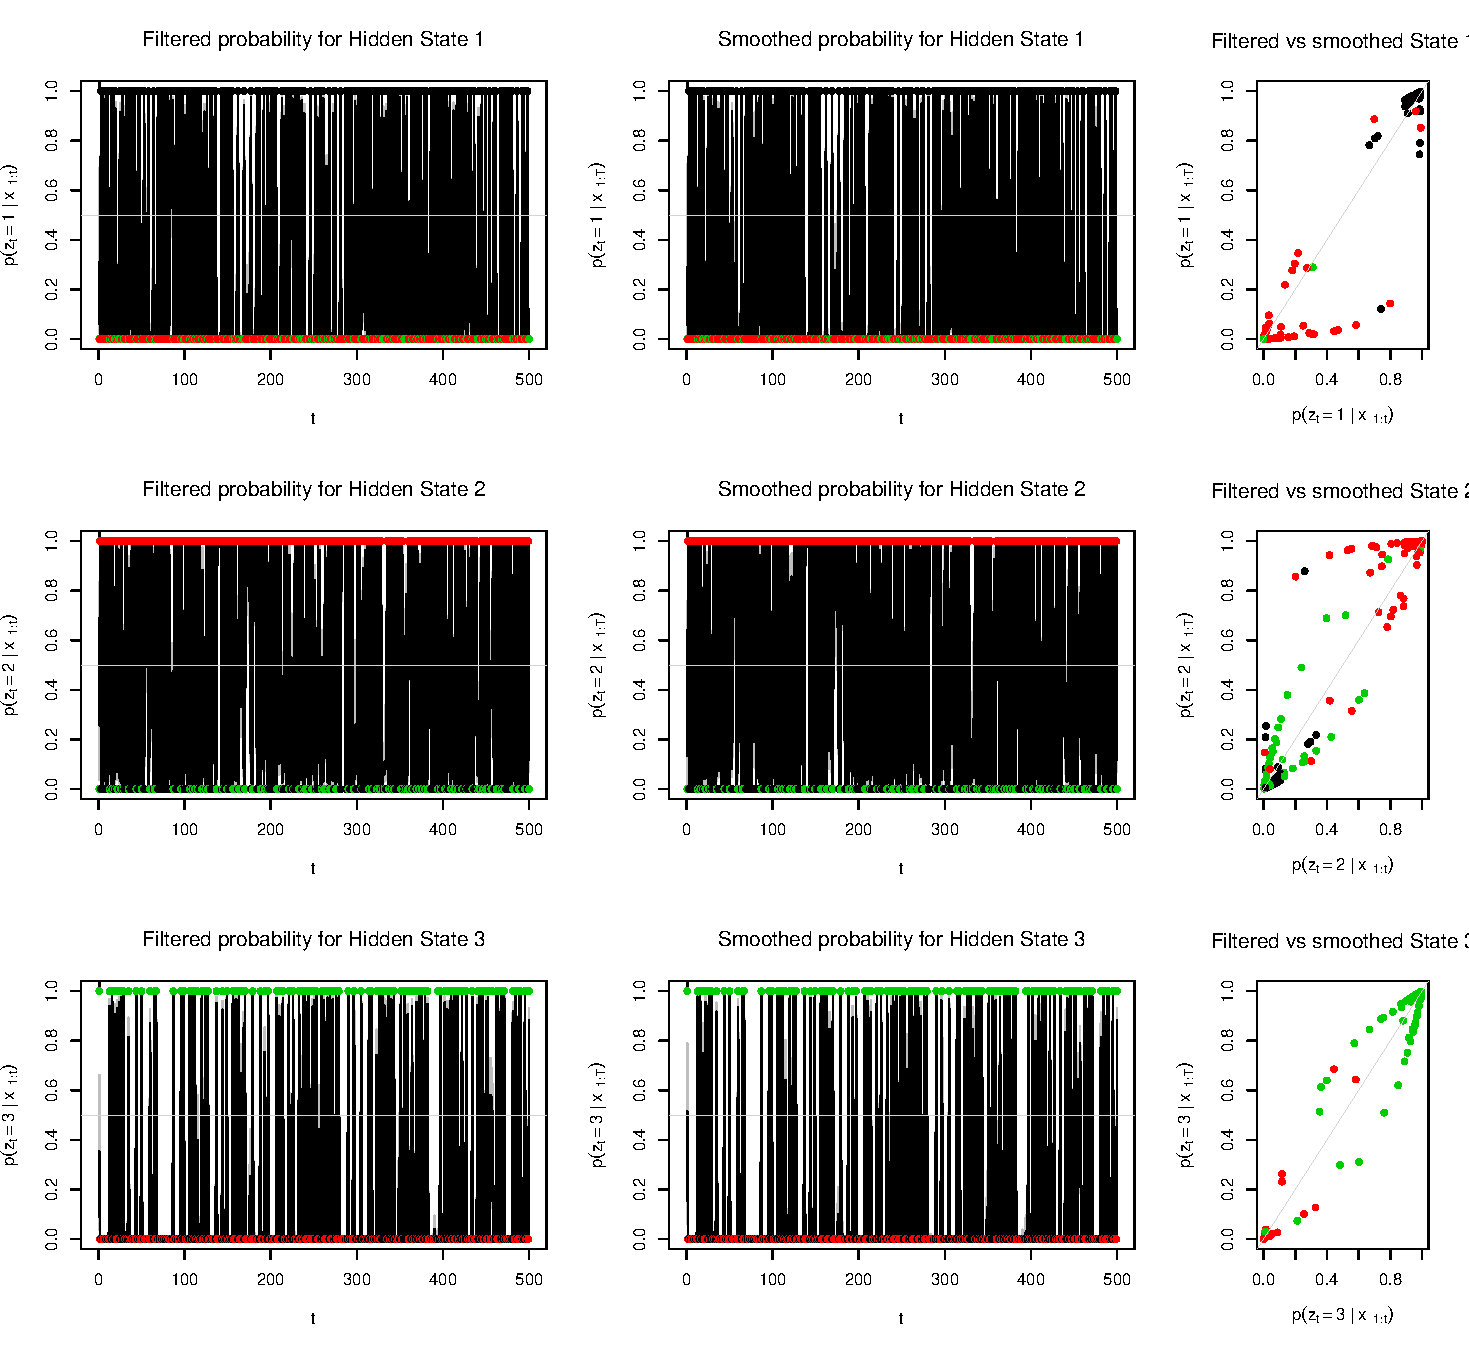
\includegraphics[width=\textwidth]{main_pdf_files/figure-latex/hmm_walkthrough_stateprobability-1}

We identify an insignificant quantity of misclassifications product of
the stochastic nature of our software.

As expected, the MAP estimate recovers the simulated hidden path with no
label switching due because of the ordinal constraints.

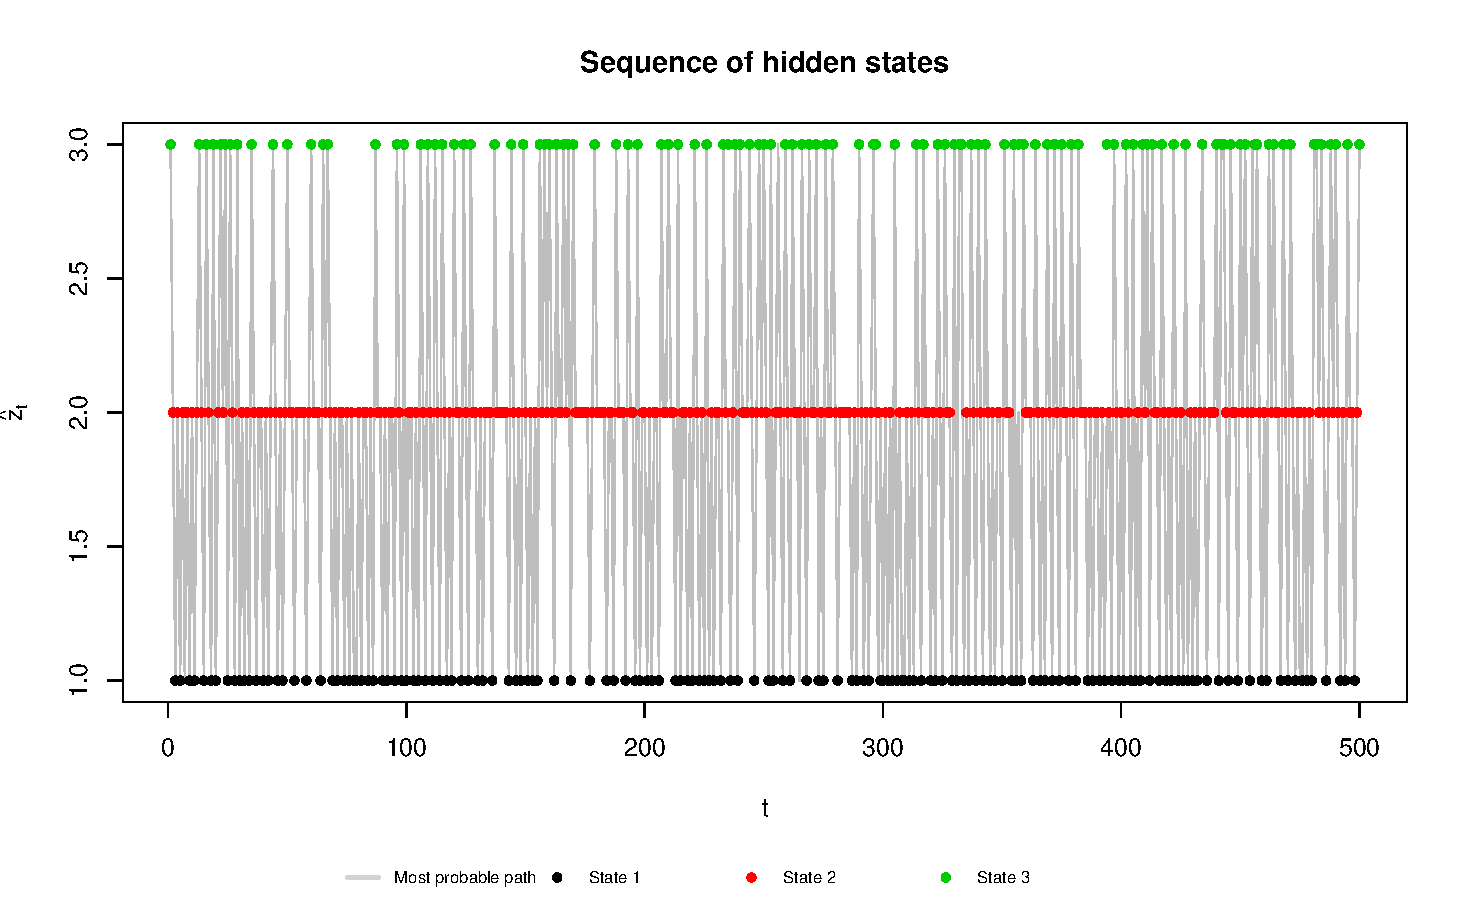
\includegraphics[width=\textwidth]{main_pdf_files/figure-latex/hmm_walkthrough_statepath-1}

\begin{longtable}[]{@{}lrrr@{}}
\caption{Hard classification according to the Viterbi
Algorithm.}\tabularnewline
\toprule
& \(\hat{z}_t = 1\) & \(\hat{z}_t = 2\) &
\(\hat{z}_t = 2\)\tabularnewline
\midrule
\endfirsthead
\toprule
& \(\hat{z}_t = 1\) & \(\hat{z}_t = 2\) &
\(\hat{z}_t = 2\)\tabularnewline
\midrule
\endhead
\(z_t = 1\) & 154 & 1 & 0\tabularnewline
\(z_t = 2\) & 4 & 227 & 2\tabularnewline
\(z_t = 3\) & 0 & 5 & 107\tabularnewline
\bottomrule
\end{longtable}

Finally, we plot the observed series colored according to the jointly
most likely state.

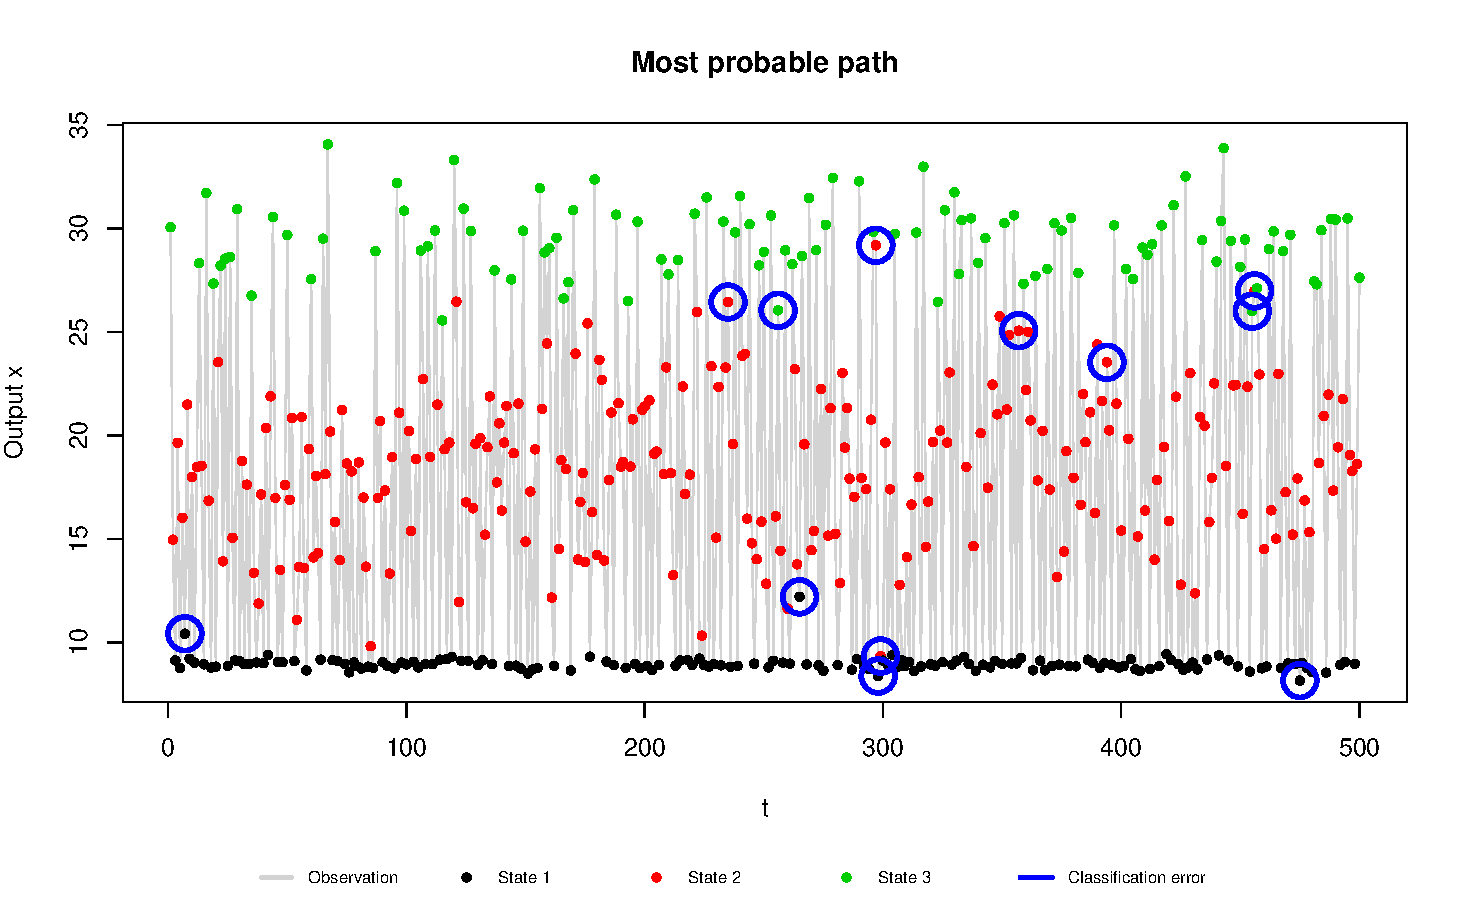
\includegraphics[width=\textwidth]{main_pdf_files/figure-latex/hmm_walkthrough_outputvit-1}

\section{The Input-Output Hidden Markov
Model}\label{the-input-output-hidden-markov-model}

The IOHMM is an architecture proposed by Bengio and Frasconi (1995) to
map input sequences, sometimes called the control signal, to output
sequences. It is a probabilistic framework that can deal with general
sequence processing tasks such as production, classification and
prediction. The main difference with Hidden Markov Models (HMM), which
are part of the unsupervised learning paradigm, is the capability to
learn the output sequence itself instead of the distribution of the
output sequence.

\subsection{Definitions}\label{definitions}

As with HMM, IOHMM involves two interconnected models,

\begin{align*}
z_{t} &= f(z_{t-1}, \mat{u}_{t}) \\
\mat{x}_{t} &= g(z_{t  }, \mat{u}_{t}).
\end{align*}

The first line corresponds to the state model, which consists of
discrete-time, discrete-state hidden states \(z_t \in \{1, \dots, K\}\)
whose transition depends on the previous hidden state \(z_{t-1}\) and
the input vector \(\mat{u}_{t} \in \RR^M\). Additionally, the
observation model is governed by \(g(z_{t}, \mat{u}_{t})\), where
\(\mat{x}_t \in \RR^R\) is the vector of observations, emissions or
output. The corresponding joint distribution is

\[
p(\mat{z}_{1:T}, \mat{x}_{1:T} | \mat{u}_{t}).
\]

In the proposed parametrization with continuous inputs and outputs, the
state model involves a multinomial regression whose parameters depend on
the previous state taking the value \(i\),

\[
p(z_t | \mat{x}_{t}, \mat{u}_{t}, z_{t-1} = i) = \text{softmax}^{-1}(\mat{u}_{t} \mat{w}_i),
\]

and the observation model is built upon a linear regression with
Gaussian error and parameters depending on the current state taking the
value \(j\),

\[
p(\mat{x}_t | \mat{u}_{t}, z_{t} = j) = \mathcal{N}(\mat{u}_t \mat{b}_j, \mat{\Sigma}_j)
\]

IOHMM adapts the logic of HMM to allow for input and output vectors,
retaining its fully probabilistic quality. Hidden states are assumed to
follow a multinomial distribution that depends on the input sequence.
The transition probabilities
\(\Psi_t(i, j) = p(z_t = j | z_{t-1} = i, \mat{u}_{t})\), which govern
the state dynamics, are driven by the control signal as well.

As for the output sequence, the local evidence at time \(t\) now becomes
\(\psi_t(j) = p(\mat{x}_t | z_t = j, \mat{\eta}_t)\), where
\(\mat{\eta}_t = \ev{\mat{x}_t | z_t, \mat{u}_t}\) can be interpreted as
the expected location parameter for the probability distribution of the
emission \(\mat{x}_{t}\) conditional on the input vector \(\mat{u}_t\)
and the hidden state \(z_t\).

The actual form of the emission density \(p(\mat{x}_t, \mat{\eta}_t)\)
can be discrete or continuous. In case of sequence classification or
symbolic mutually exclusive emissions, it is possible to set up the
multinomial distribution by running the softmax function over the
estimated outputs of all possible states. In this case, we approximate
continuous observations with the Gaussian density, the target is
estimated as a linear combination of these outputs.

The adaptation of the data and parameters blocks is straightforward: we
add the number of input variables \texttt{M}, the array of input vectors
\texttt{u\_t}, the regressors \texttt{b\_km} and the residual standard
deviation \texttt{s\_k}.

\begin{verbatim}
data {
  int<lower=1> T;                   // number of observations (length)
  int<lower=1> K;                   // number of hidden states
  int<lower=1> M;                   // size of the input vector

  real x_t[T];                      // output (scalar so far)
  vector[M] u[T];                // input vectors
}

parameters {
  // Discrete state model
  simplex[K] pi1;                  // initial state probabilities
  vector[M] w[K];                // state regressors

  // Continuous observation model
  vector[M] b[K];                // mean regressors
  real<lower=0.0001> sigma[K];        // residual standard deviations
}
\end{verbatim}

\subsection{Inference}\label{inference-1}

\subsubsection{Filtering}\label{filtering-1}

The filtered marginals are computed recursively by adjusting the forward
algorithm to consider the input sequence,

\begin{align*}
\alpha_t(j)
  & \triangleq p(z_t = j | \mat{x}_{1:t}, \mat{u}_{1:t}) \\
  & = \sum_{i = 1}^{K}{p(z_t = j | z_{t-1} = i, \mat{x}_{t}, \mat{u}_{t}) p(z_{t-1} = i | \mat{x}_{1:t-1}, \mat{u}_{1:t-1})} \\
  & = \sum_{i = 1}^{K}{p(\mat{x}_{t} | z_t = j, \mat{u}_t) p(z_t = j | z_{t-1} = i, \mat{u}_{t}) p(z_{t-1} = i | \mat{x}_{1:t-1}, \mat{u}_{1:t-1})} \\
  & = \psi_t(j) \sum_{i = 1}^{K}{\Psi_t(i, j) \alpha_{t-1}(i)}.
\end{align*}

The implementation in Stan requires one modification: the time-dependent
transition probability matrix is now computed as the linear combination
of the input variables and the parameters of the multinomial regression
that drives the latent process.

\begin{verbatim}
transformed parameters {
  vector[K] logalpha[T];

  vector[K] unA[T];
  vector[K] A[T];

  vector[K] logoblik[T];

  { // Transition probability matrix p(z_t = j | z_{t-1} = i, u)
    unA[1] = pi1; // Filler
    A[1] = pi1; // Filler
    for (t in 2:T) {
      for (j in 1:K) { // j = current (t)
        unA[t][j] = u[t]' * w[j];
      }
      A[t] = softmax(unA[t]);
    }
  }

  { // Evidence (observation likelihood)
    for(t in 1:T) {
      for(j in 1:K) {
        logoblik[t][j] = normal_lpdf(x_t[t] | mu[j], sigma[j]);
      }
    }
  }

  { // Forward algorithm log p(z_t = j | x_{1:t})
    real accumulator[K];

    for(j in 1:K)
      logalpha[1][j] = log(pi1[j]) + logoblik[1][j];

    for (t in 2:T) {
      for (j in 1:K) { // j = current (t)
        for (i in 1:K) { // i = previous (t-1)
                         // Murphy (2012) Eq. 17.48
                         // belief state + transition prob + local evidence at t
          accumulator[i] = logalpha[t-1, i] 
                           + log(A[t][i]) 
                           + logoblik[t][j];
        }
        logalpha[t, j] = log_sum_exp(accumulator);
      }
    }
  } // Forward
}
\end{verbatim}

\subsubsection{Smoothing}\label{smoothing-1}

A smoother infers the belief state at a given step based on all the
observations or evidence,

\begin{align*}
\gamma_t(j)
  & \triangleq p(z_t = j | \mat{x}_{1:T}, \mat{u}_{1:T}) \\
  & \propto \alpha_t(j) \beta_t(j),
\end{align*}

where

\begin{align*}
\beta_{t-1}(i)
  & \triangleq p(\mat{x}_{t:T} | z_{t-1} = i, \mat{u}_{t:T}).
\end{align*}

Similarly, inference about the smoothed posterior marginal requires the
adaptation of the forward-backward algorithm to consider the input
sequence in both components \(\alpha_t(j)\) and \(\beta_t(j)\). The
latter now becomes

\begin{align*}
\beta_{t-1}(i)
  & \triangleq p(\mat{x}_{t:T} | z_{t-1} = i, \mat{u}_{t:T}) \\
  & = \sum_{j = 1}^{K}{\psi_t(j) \Psi_t(i, j) \beta_{t}(j)}.
\end{align*}

Once adjusted the transition probability matrix, the Stan code for the
forward-backward algorithm need no further modification.

\subsubsection{MAP: Viterbi}\label{map-viterbi-1}

The Stan code for the Viterbi encoding algorithm need no further
modification.

\subsection{Parameter estimation}\label{parameter-estimation-1}

The parameters of the models are
\(\mat{\theta} = (\mat{\pi}_1, \mat{\theta}_h, \mat{\theta}_o)\), where
\(\mat{\pi}_1\) is the initial state distribution, \(\mat{\theta}_h\)
are the parameters of the hidden model and \(\mat{\theta}_o\) are the
parameters of the state-conditional density function
\(p(\mat{x}_t | z_t = j, \mat{u}_t)\). State transition is characterized
by a multinomial regression with parameters \(\mat{w}_k\) for
\(k \in \{1, \dots, K\}\), while emissions are modeled by a linear
regression with Gaussian error and parameters \(\mat{b}_k\) and
\(\mat{\Sigma}_k\) for \(k \in \{1, \dots, K\}\).

Estimation can be run under both the maximum likelihood and Bayesian
frameworks. Although it is a straightforward procedure when the data is
fully observed, in practice the latent states \(\mat{z}_{1:T}\) are
hidden. The most common approach is the application of the EM algorithm
to find either the maximum likelihood or the maximum a posteriori
estimates. Bengio and Frasconi (1995) proposes a straightforward
modification of the EM algorithm. The application of sigmoidal
functions, for example the logistic or softmax transforms for the hidden
transition model, requires numeric optimization via gradient ascent or
similar methods for the M step. In this work, we exploit Stan's
capabilities to produce a sampler that explores the posterior density of
the model parameters.

\subsection{A walk-though the IOHMM}\label{a-walk-though-the-iohmm}

\subsubsection{Numerical stability for the softmax
function}\label{numerical-stability-for-the-softmax-function}

A digression! The softmax function, or normalized exponential function,
can suffer from over or underflow in the exponentials. A naive
implementation may fail:

\begin{Shaded}
\begin{Highlighting}[]
\NormalTok{x <-}\StringTok{ }\DecValTok{10}\NormalTok{^(}\DecValTok{1}\NormalTok{:}\DecValTok{5}\NormalTok{)}
\KeywordTok{exp}\NormalTok{(x) /}\StringTok{ }\KeywordTok{sum}\NormalTok{(}\KeywordTok{exp}\NormalTok{(x))}
\end{Highlighting}
\end{Shaded}

\begin{verbatim}
## [1]   0   0 NaN NaN NaN
\end{verbatim}

A well known, safer implementation exploits the fact that softmax is
location invariant, ie \(softmax(\mat{x}) = softmax(\mat{x} + c)\) for
any constant \(c\). Subtracting the maximum value produces a new vector
with non-positive entries, ruling out overflows, and at least one zero
element, guaranteeing at least one significant term in the denominator.

\begin{Shaded}
\begin{Highlighting}[]
\NormalTok{logsumexp <-}\StringTok{ }\NormalTok{function(x) \{}
  \NormalTok{y =}\StringTok{ }\KeywordTok{max}\NormalTok{(x)}
  \NormalTok{y +}\StringTok{ }\KeywordTok{log}\NormalTok{(}\KeywordTok{sum}\NormalTok{(}\KeywordTok{exp}\NormalTok{(x -}\StringTok{ }\NormalTok{y)))}
\NormalTok{\}}

\NormalTok{softmax <-}\StringTok{ }\NormalTok{function(x) \{}
  \KeywordTok{exp}\NormalTok{(x -}\StringTok{ }\KeywordTok{logsumexp}\NormalTok{(x))}
\NormalTok{\}}

\KeywordTok{softmax}\NormalTok{(x)}
\end{Highlighting}
\end{Shaded}

\begin{verbatim}
## [1] 0 0 0 0 1
\end{verbatim}

This is already taken care in Stan (Stan Development Team 2017c, 474).

\subsubsection{Back to the walk-though}\label{back-to-the-walk-though}

We first adapt the R routine for our new generative model. The arguments
are the sequence length \(T\), the number of discrete hidden states
\(K\), the input matrix \(\mat{u}\), the initial state distribution
vector \(\mat{\pi}_1\), a matrix with the parameters of the multinomial
regression that rules the hidden states dynamics \(\mat{w}\), the name
of a function drawing samples from the observation distribution and its
arguments.

The initial hidden state is drawn from a multinomial distribution with
one trial and event probabilities given by the initial state probability
vector \(\mat{\pi}_1\). The transition probabilities for each of the
following steps \(t \in \{2, \dots, T\}\) are generated from a
multinomial regression with vector parameters \(\mat{w}_k\), one set per
possible hidden state \(k \in \{1, \dots, K\}\), and covariates
\(\mat{u}_t\). The hidden states are subsequently sampled based on these
transition probabilities.

The observation at each step may generate from a Gaussian with
parameters \(\mu_k\) and \(\sigma_k\), one set per possible hidden
state.

\begin{Shaded}
\begin{Highlighting}[]
\NormalTok{iohmm_generate <-}\StringTok{ }\NormalTok{function(T) \{}
  \CommentTok{# 1. Parameters}
  \NormalTok{K <-}\StringTok{ }\DecValTok{3}
  \NormalTok{M <-}\StringTok{ }\DecValTok{4}
  \NormalTok{u <-}\StringTok{ }\KeywordTok{matrix}\NormalTok{(}\KeywordTok{rnorm}\NormalTok{(T *}\StringTok{ }\NormalTok{M), }\DataTypeTok{nrow =} \NormalTok{T, }\DataTypeTok{ncol =} \NormalTok{M, }\DataTypeTok{byrow =} \OtherTok{TRUE}\NormalTok{)}
  \NormalTok{w <-}\StringTok{ }\KeywordTok{matrix}\NormalTok{(}
    \KeywordTok{c}\NormalTok{(}\FloatTok{1.2}\NormalTok{, }\FloatTok{0.5}\NormalTok{, }\FloatTok{0.3}\NormalTok{, }\FloatTok{0.1}\NormalTok{, }\FloatTok{0.5}\NormalTok{, }\FloatTok{1.2}\NormalTok{, }\FloatTok{0.3}\NormalTok{, }\FloatTok{0.1}\NormalTok{, }\FloatTok{0.5}\NormalTok{, }\FloatTok{0.1}\NormalTok{, }\FloatTok{1.2}\NormalTok{, }\FloatTok{0.1}\NormalTok{),}
    \DataTypeTok{nrow =} \NormalTok{K, }\DataTypeTok{ncol =} \NormalTok{M, }\DataTypeTok{byrow =} \OtherTok{TRUE}\NormalTok{)}
  \NormalTok{b <-}\StringTok{ }\KeywordTok{matrix}\NormalTok{(}
    \KeywordTok{c}\NormalTok{(}\FloatTok{5.0}\NormalTok{, }\FloatTok{6.0}\NormalTok{, }\FloatTok{7.0}\NormalTok{, }\FloatTok{0.5}\NormalTok{, }\FloatTok{1.0}\NormalTok{, }\FloatTok{5.0}\NormalTok{, }\FloatTok{0.1}\NormalTok{, -}\FloatTok{0.5}\NormalTok{, }\FloatTok{0.1}\NormalTok{, -}\FloatTok{1.0}\NormalTok{, -}\FloatTok{5.0}\NormalTok{, }\FloatTok{0.2}\NormalTok{),}
    \DataTypeTok{nrow =} \NormalTok{K, }\DataTypeTok{ncol =} \NormalTok{M, }\DataTypeTok{byrow =} \OtherTok{TRUE}\NormalTok{)}
  \NormalTok{sigma <-}\StringTok{ }\KeywordTok{c}\NormalTok{(}\FloatTok{0.2}\NormalTok{, }\FloatTok{1.0}\NormalTok{, }\FloatTok{2.5}\NormalTok{)}
  \NormalTok{pi1 <-}\StringTok{ }\KeywordTok{c}\NormalTok{(}\FloatTok{0.4}\NormalTok{, }\FloatTok{0.2}\NormalTok{, }\FloatTok{0.4}\NormalTok{)}
  
  \NormalTok{p.mat <-}\StringTok{ }\KeywordTok{matrix}\NormalTok{(}\DecValTok{0}\NormalTok{, }\DataTypeTok{nrow =} \NormalTok{T, }\DataTypeTok{ncol =} \NormalTok{K)}
  \NormalTok{p.mat[}\DecValTok{1}\NormalTok{, ] <-}\StringTok{ }\NormalTok{pi1}

  \CommentTok{# 2. Hidden path}
  \NormalTok{z <-}\StringTok{ }\KeywordTok{vector}\NormalTok{(}\StringTok{"numeric"}\NormalTok{, T)}
  \NormalTok{z[}\DecValTok{1}\NormalTok{] <-}\StringTok{ }\KeywordTok{sample}\NormalTok{(}\DataTypeTok{x =} \DecValTok{1}\NormalTok{:K, }\DataTypeTok{size =} \DecValTok{1}\NormalTok{, }\DataTypeTok{replace =} \OtherTok{FALSE}\NormalTok{, }\DataTypeTok{prob =} \NormalTok{pi1)}
  \NormalTok{for (t in }\DecValTok{2}\NormalTok{:T) \{}
    \NormalTok{p.mat[t, ] <-}\StringTok{ }\KeywordTok{softmax}\NormalTok{(}\KeywordTok{sapply}\NormalTok{(}\DecValTok{1}\NormalTok{:K, function(j) \{u[t, ] %*%}\StringTok{ }\NormalTok{w[j, ]\}))}
    \NormalTok{z[t] <-}\StringTok{ }\KeywordTok{sample}\NormalTok{(}\DataTypeTok{x =} \DecValTok{1}\NormalTok{:K, }\DataTypeTok{size =} \DecValTok{1}\NormalTok{, }\DataTypeTok{replace =} \OtherTok{FALSE}\NormalTok{, }\DataTypeTok{prob =} \NormalTok{p.mat[t, ])}
  \NormalTok{\}}

  \CommentTok{# 3. Observations}
  \NormalTok{x_t <-}\StringTok{ }\KeywordTok{vector}\NormalTok{(}\StringTok{"numeric"}\NormalTok{, T)}
  \NormalTok{for (t in }\DecValTok{1}\NormalTok{:T) \{}
    \NormalTok{x_t[t] <-}\StringTok{ }\KeywordTok{rnorm}\NormalTok{(}\DecValTok{1}\NormalTok{, u[t, ] %*%}\StringTok{ }\NormalTok{b[z[t], ], sigma[z[t]])}
  \NormalTok{\}}

  \KeywordTok{list}\NormalTok{(}
    \DataTypeTok{u =} \NormalTok{u,}
    \DataTypeTok{z_t =} \NormalTok{z_t,}
    \DataTypeTok{x_t =} \NormalTok{x_t,}
    \DataTypeTok{theta =} \KeywordTok{list}\NormalTok{(}\DataTypeTok{pi1 =} \NormalTok{pi1, }\DataTypeTok{w =} \NormalTok{w,}
                 \DataTypeTok{b =} \NormalTok{b, }\DataTypeTok{sigma =} \NormalTok{sigma, }\DataTypeTok{p.mat =} \NormalTok{p.mat)}
  \NormalTok{)}
\NormalTok{\}}
\end{Highlighting}
\end{Shaded}

We draw one sample of length \(T=500\) from a data generating process
with \(K=3\) latent states and run an exploratory analysis of the
observed quantities.

\begin{Shaded}
\begin{Highlighting}[]
\KeywordTok{set.seed}\NormalTok{(}\DecValTok{900}\NormalTok{)}
\NormalTok{K <-}\StringTok{ }\DecValTok{3}
\NormalTok{T_length <-}\StringTok{ }\DecValTok{500}
\NormalTok{dataset  <-}\StringTok{ }\KeywordTok{iohmm_generate}\NormalTok{(T_length)}
\end{Highlighting}
\end{Shaded}

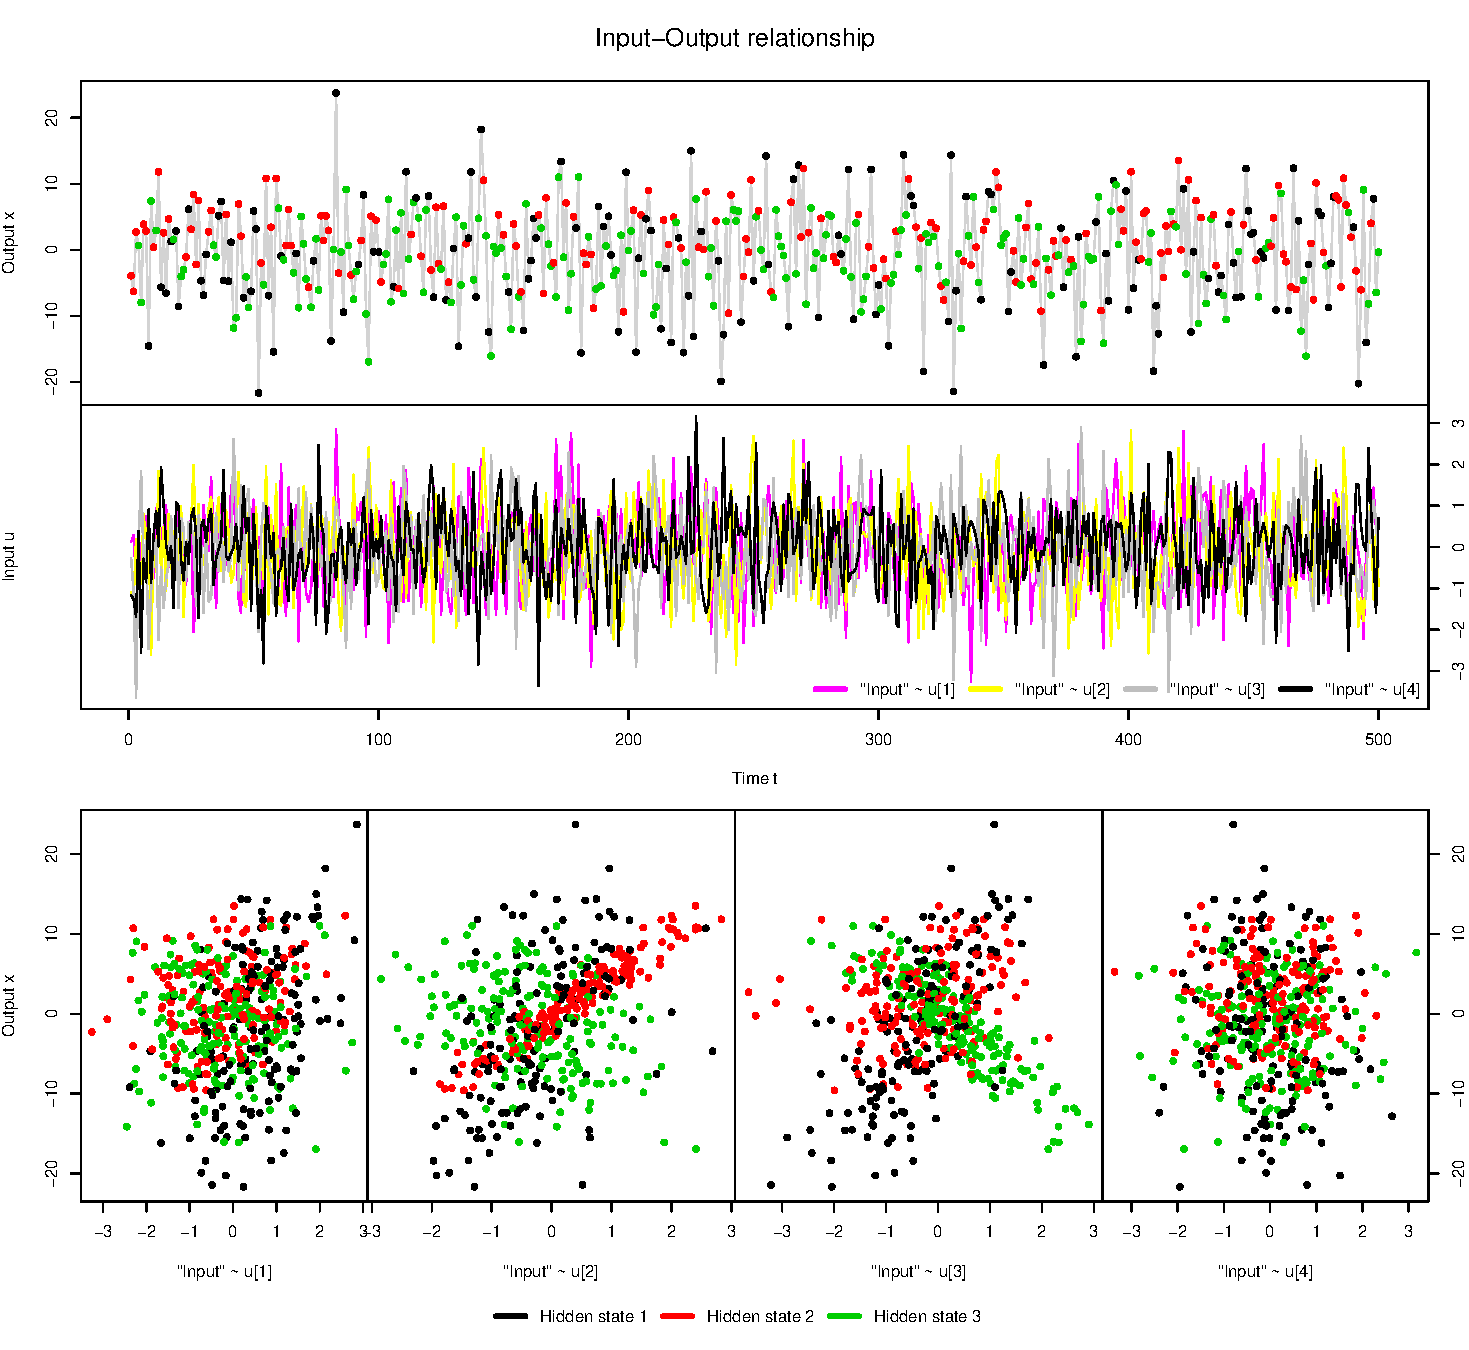
\includegraphics[width=\textwidth]{main_pdf_files/figure-latex/iohmm_walkthrough_inputoutput-1}

We observe how the chosen values for the parameters affect the generated
data. For example, the relationship between the third input
\(\mat{u}_3\) and the output \(\mat{x}_t\) is positive, indifferent and
negative for the hidden states \(K = 1, 2, 3\) respectively. The true
slopes are 7, 0.1 and -5.

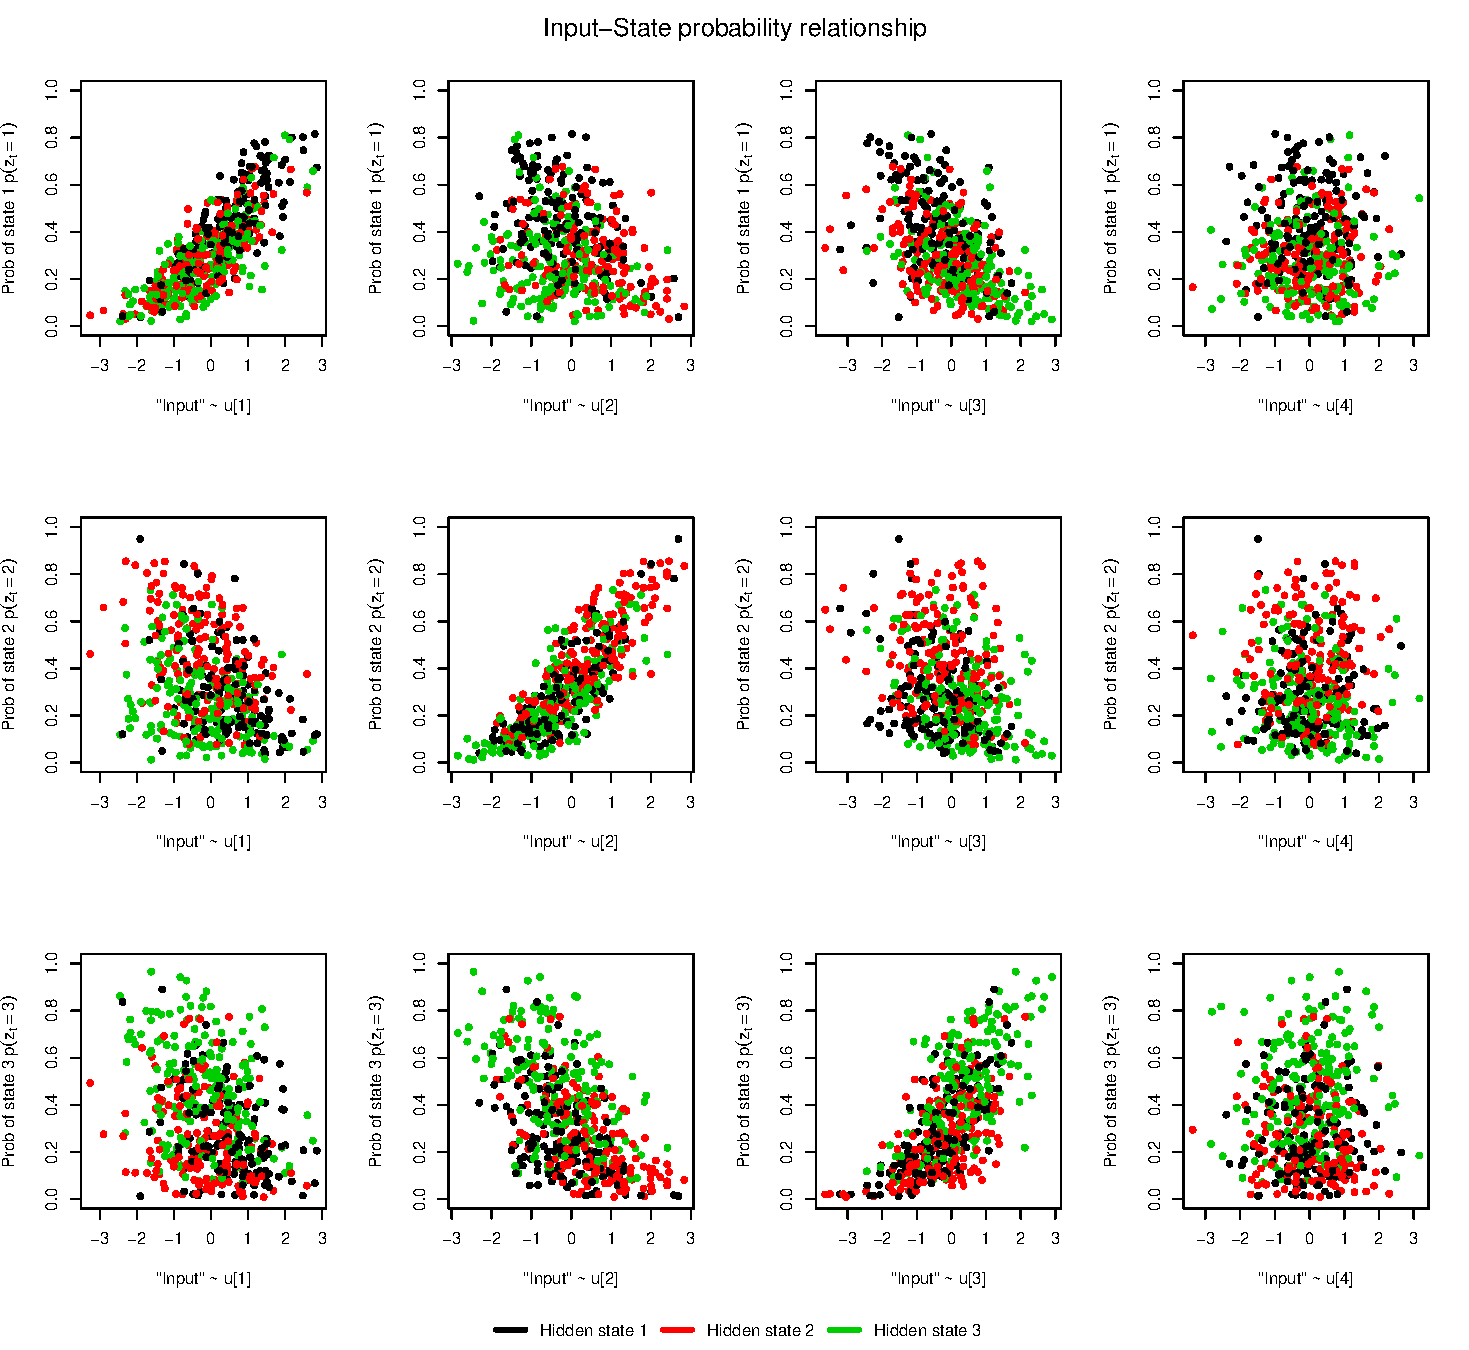
\includegraphics[width=\textwidth]{main_pdf_files/figure-latex/iohmm_walkthrough_inputprob-1}

We then analyse the relationship between the input and the state
probabilities, which are usually hidden in applications with real data.
The pairs \(\{ \mat{u}_1, p(z_t = 1) \}\),
\(\{ \mat{u}_2, p(z_t = 2) \}\) and \(\{ \mat{u}_3, p(z_t = 3) \}\) show
the strongest relationships because of values of true regression
parameters: those inputs take the largest weight in each state, namely
\(w_{11} = 1.2\), \(w_{22} = 1.2\) and \(w_{33} = 1.2\).

We run the software to draw samples from the posterior density of model
parameters and other hidden quantities.

We rely on several diagnostic statistics and plots provided by rstan
(Stan Development Team 2017a) and shinystan (Stan Development Team
2017b) to assess mixing, convergence and the absence of divergences.
Label switching hinders the comparison between true and observed
parameters.

\begin{longtable}[]{@{}lrrrrrrrrr@{}}
\caption{Estimated parameters and hidden quantities. \emph{MCSE = Monte
Carlo Standard Error, SE = Standard Error, ESS = Effective Sample
Size}.}\tabularnewline
\toprule
& True & Mean & MCSE & SE & \(q_{10\%}\) & \(q_{50\%}\) & \(q_{90\%}\) &
ESS & \(\hat{R}\)\tabularnewline
\midrule
\endfirsthead
\toprule
& True & Mean & MCSE & SE & \(q_{10\%}\) & \(q_{50\%}\) & \(q_{90\%}\) &
ESS & \(\hat{R}\)\tabularnewline
\midrule
\endhead
p\_1k{[}1{]} & 0.4 & 0.24 & 0.01 & 0.18 & 0.04 & 0.20 & 0.50 & 200.00 &
1.00\tabularnewline
p\_1k{[}2{]} & 0.2 & 0.26 & 0.01 & 0.19 & 0.05 & 0.23 & 0.54 & 200.00 &
1.00\tabularnewline
p\_1k{[}3{]} & 0.4 & 0.50 & 0.02 & 0.22 & 0.20 & 0.49 & 0.79 & 200.00 &
1.00\tabularnewline
w\_km{[}1,1{]} & 1.2 & -0.06 & 0.25 & 2.71 & -3.74 & 0.46 & 3.13 &
121.58 & 1.00\tabularnewline
w\_km{[}1,2{]} & 0.5 & -0.05 & 0.21 & 2.87 & -3.55 & -0.08 & 3.82 &
189.90 & 1.02\tabularnewline
w\_km{[}1,3{]} & 0.3 & -0.07 & 0.31 & 2.92 & -3.75 & -0.26 & 3.69 &
91.49 & 1.00\tabularnewline
w\_km{[}1,4{]} & 0.1 & 0.44 & 0.23 & 2.61 & -3.14 & 0.37 & 3.55 & 128.73
& 1.00\tabularnewline
w\_km{[}2,1{]} & 0.5 & -0.06 & 0.25 & 2.72 & -3.73 & 0.48 & 3.13 &
120.68 & 1.00\tabularnewline
w\_km{[}2,2{]} & 1.2 & -0.13 & 0.21 & 2.85 & -3.75 & -0.22 & 3.73 &
189.58 & 1.01\tabularnewline
w\_km{[}2,3{]} & 0.3 & -0.07 & 0.31 & 2.92 & -3.80 & -0.26 & 3.60 &
90.67 & 1.00\tabularnewline
w\_km{[}2,4{]} & 0.1 & 0.58 & 0.23 & 2.60 & -3.02 & 0.61 & 3.74 & 129.67
& 1.00\tabularnewline
w\_km{[}3,1{]} & 0.5 & -0.25 & 0.25 & 2.73 & -4.01 & 0.33 & 3.01 &
120.45 & 1.00\tabularnewline
w\_km{[}3,2{]} & 0.1 & -0.09 & 0.21 & 2.86 & -3.62 & -0.15 & 3.72 &
189.68 & 1.01\tabularnewline
w\_km{[}3,3{]} & 1.2 & -0.09 & 0.31 & 2.93 & -3.80 & -0.28 & 3.62 &
90.45 & 1.00\tabularnewline
w\_km{[}3,4{]} & 0.1 & 0.48 & 0.23 & 2.59 & -3.07 & 0.46 & 3.64 & 130.86
& 1.00\tabularnewline
b\_km{[}1,1{]} & 5.0 & -0.04 & 0.02 & 0.24 & -0.35 & -0.03 & 0.25 &
200.00 & 1.00\tabularnewline
b\_km{[}1,2{]} & 1.0 & -1.11 & 0.01 & 0.18 & -1.33 & -1.11 & -0.88 &
200.00 & 1.00\tabularnewline
b\_km{[}1,3{]} & 0.1 & -4.91 & 0.01 & 0.19 & -5.12 & -4.93 & -4.66 &
200.00 & 1.00\tabularnewline
b\_km{[}1,4{]} & 6.0 & 0.15 & 0.02 & 0.21 & -0.10 & 0.14 & 0.42 & 200.00
& 1.00\tabularnewline
b\_km{[}2,1{]} & 5.0 & 4.98 & 0.00 & 0.02 & 4.97 & 4.98 & 5.00 & 200.00
& 1.00\tabularnewline
b\_km{[}2,2{]} & -1.0 & 5.99 & 0.00 & 0.02 & 5.97 & 5.99 & 6.01 & 200.00
& 1.00\tabularnewline
b\_km{[}2,3{]} & 7.0 & 7.00 & 0.00 & 0.02 & 6.98 & 7.00 & 7.02 & 200.00
& 1.00\tabularnewline
b\_km{[}2,4{]} & 0.1 & 0.49 & 0.00 & 0.02 & 0.47 & 0.49 & 0.51 & 200.00
& 1.00\tabularnewline
b\_km{[}3,1{]} & -5.0 & 0.98 & 0.01 & 0.09 & 0.88 & 0.98 & 1.11 & 200.00
& 1.00\tabularnewline
b\_km{[}3,2{]} & 0.5 & 4.99 & 0.01 & 0.09 & 4.88 & 4.99 & 5.11 & 200.00
& 1.01\tabularnewline
b\_km{[}3,3{]} & -0.5 & 0.10 & 0.01 & 0.09 & -0.02 & 0.11 & 0.21 &
173.97 & 1.00\tabularnewline
b\_km{[}3,4{]} & 0.2 & -0.59 & 0.01 & 0.10 & -0.73 & -0.60 & -0.46 &
200.00 & 1.01\tabularnewline
sigma\_k{[}1{]} & 0.2 & 2.61 & 0.01 & 0.17 & 2.40 & 2.60 & 2.83 & 200.00
& 0.99\tabularnewline
sigma\_k{[}2{]} & 1.0 & 0.20 & 0.00 & 0.01 & 0.18 & 0.20 & 0.22 & 200.00
& 1.00\tabularnewline
sigma\_k{[}3{]} & 2.5 & 1.07 & 0.01 & 0.07 & 0.98 & 1.07 & 1.17 & 200.00
& 1.00\tabularnewline
\bottomrule
\end{longtable}

While mixing and convergence is extremely efficient, as expected when
dealing with generated data, we note that the regression parameters for
the latent states are the worst performers. The smaller effective size
translates into higher Monte Carlo standard error and broader
credibility intervals. One possible reason is that softmax is invariant
to change in location, thus the parameters of a multinomial regression
do not have a natural center and become harder to estimate.

We assess that our software recover the hidden states correctly. Due to
label switching, the states generated under the labels 1 through 3 were
recovered in a different order. In consequence, we decide to relabel the
observations based on the best fit. This would not pose an inconvenient
with real data as the hidden states are never observed.

\begin{longtable}[]{@{}lrrr@{}}
\caption{Simulated hidden states are relabeled to match the order of the
recovered states.}\tabularnewline
\toprule
& \(z_1\) & \(z_2\) & \(z_3\)\tabularnewline
\midrule
\endfirsthead
\toprule
& \(z_1\) & \(z_2\) & \(z_3\)\tabularnewline
\midrule
\endhead
\(z^r_1\) & 0 & 0 & 183\tabularnewline
\(z^r_2\) & 152 & 0 & 0\tabularnewline
\(z^r_3\) & 0 & 165 & 0\tabularnewline
\bottomrule
\end{longtable}

The filtered probability is overly accurate, as expected, making the
additional information contained in the smoothed seem of little value.

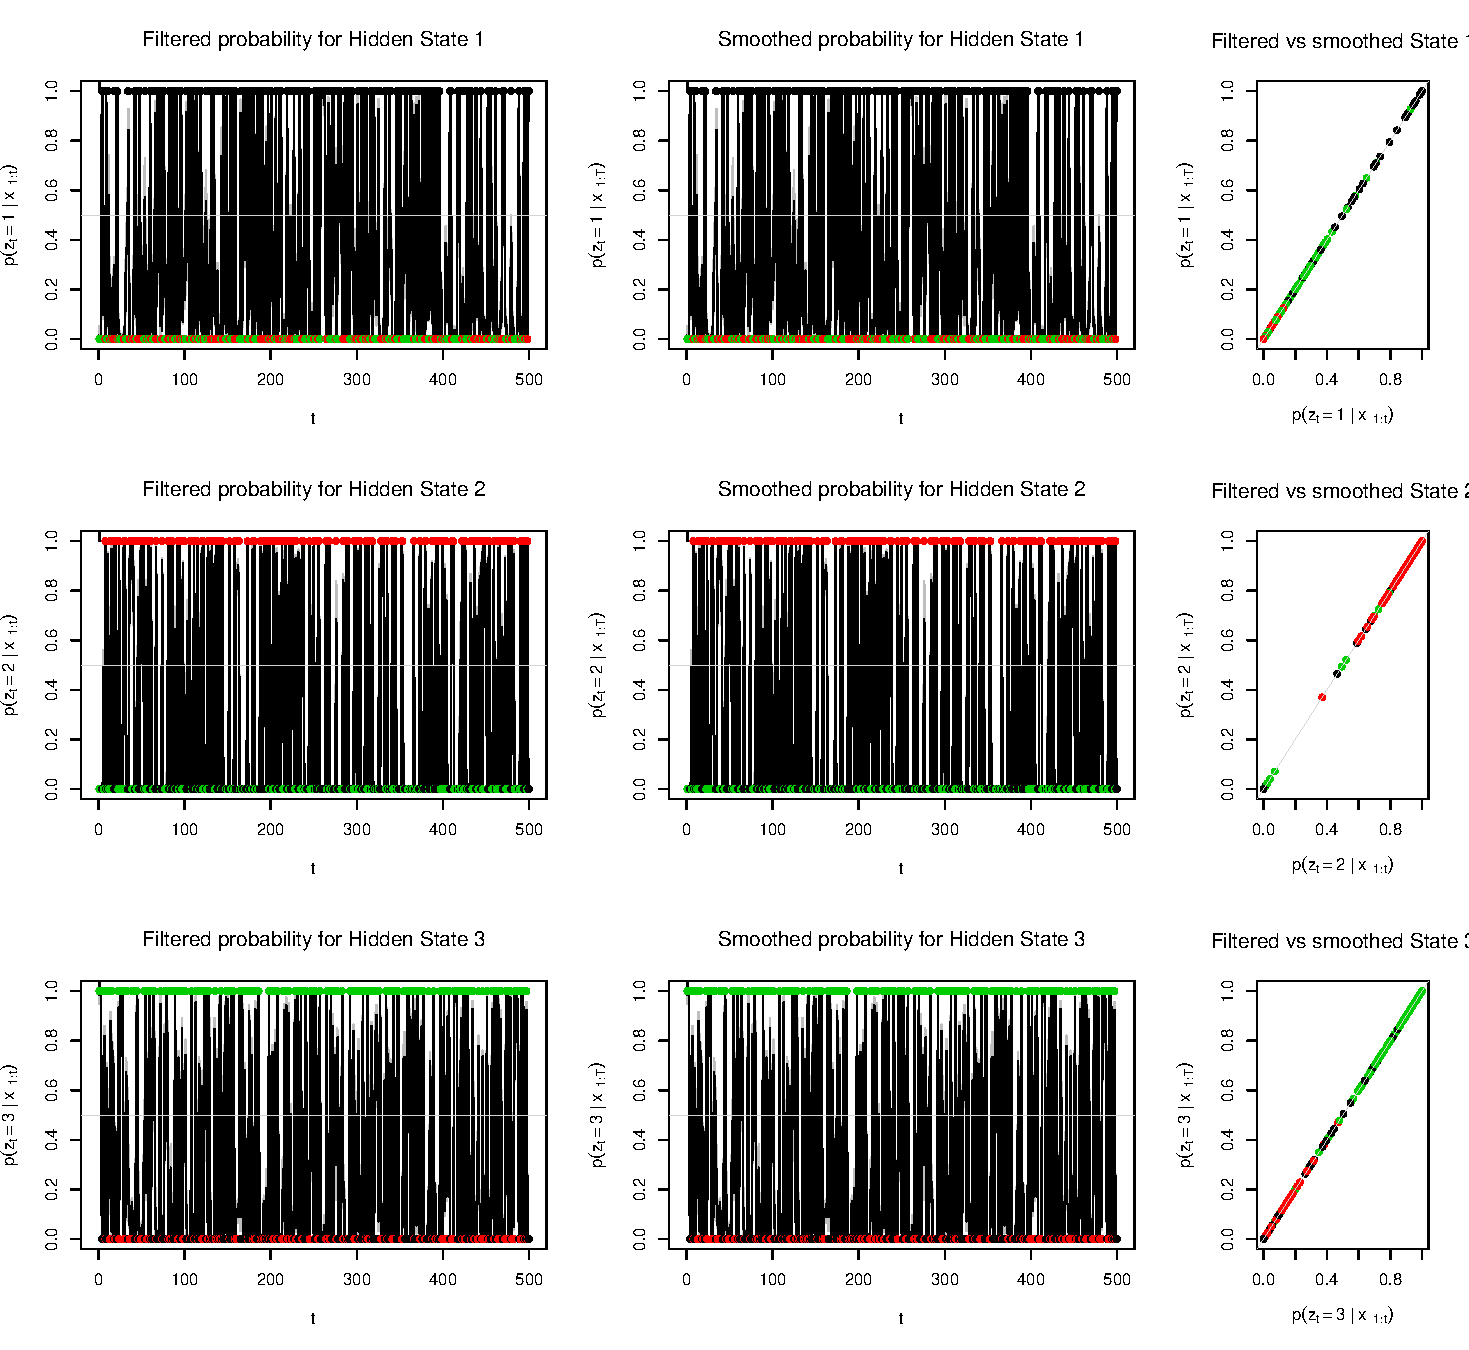
\includegraphics[width=\textwidth]{main_pdf_files/figure-latex/iohmm_walkthrough_stateprobability-1}

The confusion matrix makes evident that, under ideal conditions, the
sampler works as intended.

\begin{longtable}[]{@{}lrrr@{}}
\caption{Hard classification according to the filtered
probability.}\tabularnewline
\toprule
& \(\hat{z}_t = 1\) & \(\hat{z}_t = 2\) &
\(\hat{z}_t = 2\)\tabularnewline
\midrule
\endfirsthead
\toprule
& \(\hat{z}_t = 1\) & \(\hat{z}_t = 2\) &
\(\hat{z}_t = 2\)\tabularnewline
\midrule
\endhead
\(z^r_t = 1\) & 155 & 1 & 6\tabularnewline
\(z^r_t = 2\) & 6 & 151 & 7\tabularnewline
\(z^r_t = 3\) & 22 & 0 & 152\tabularnewline
\bottomrule
\end{longtable}

Similarly, the Viterbi algorithm recovers the expected most probably
hidden state.

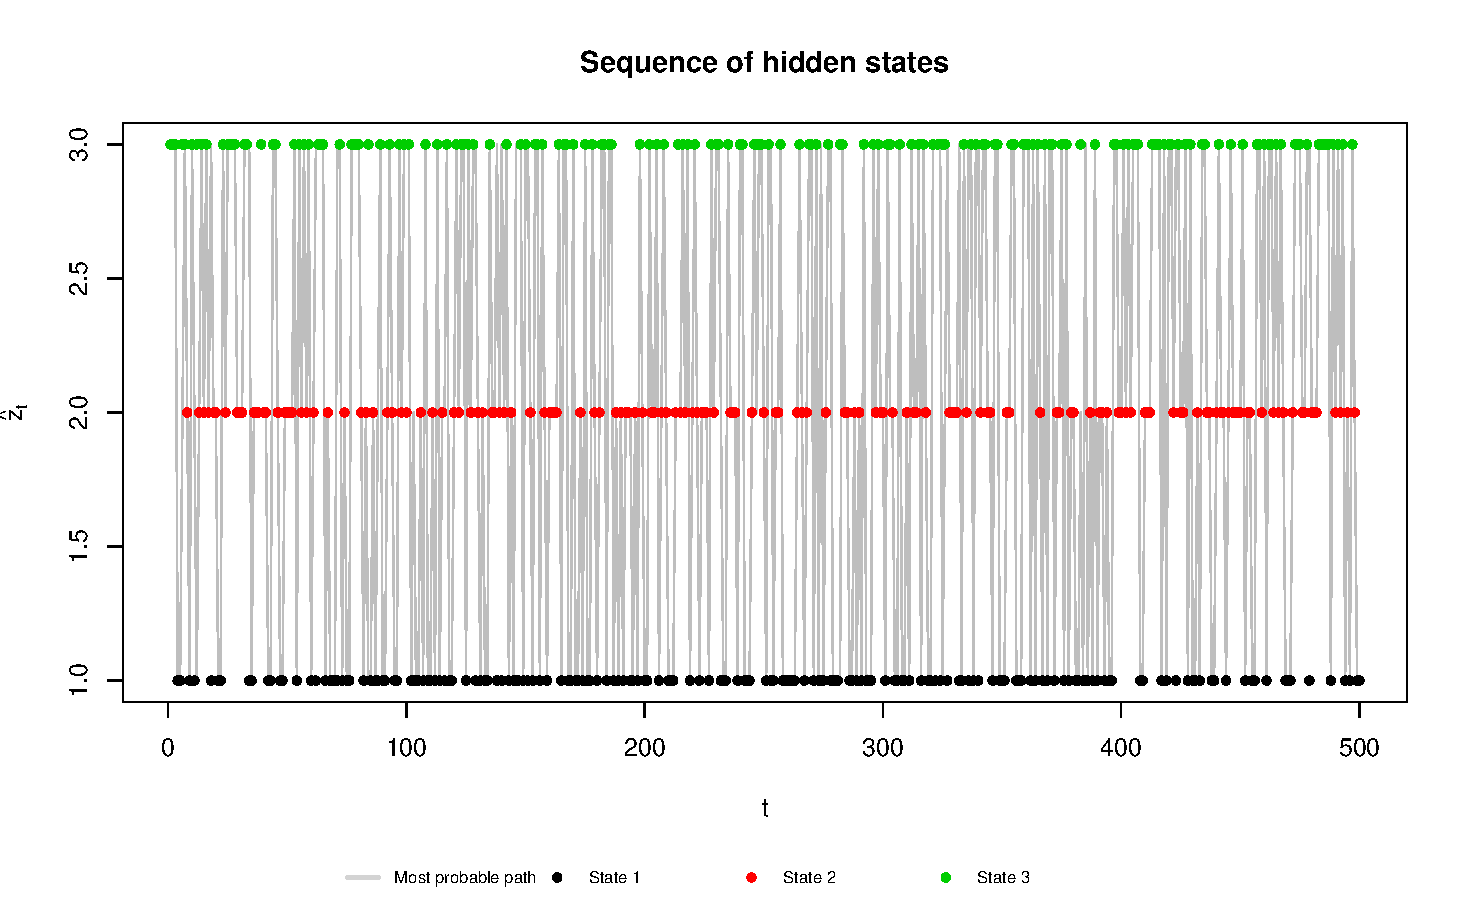
\includegraphics[width=\textwidth]{main_pdf_files/figure-latex/iohmm_walkthrough_statepath-1}

\begin{longtable}[]{@{}lrrr@{}}
\caption{Hard classification according to the Viterbi
Algorithm.}\tabularnewline
\toprule
& \(\hat{z}_t = 1\) & \(\hat{z}_t = 2\) &
\(\hat{z}_t = 2\)\tabularnewline
\midrule
\endfirsthead
\toprule
& \(\hat{z}_t = 1\) & \(\hat{z}_t = 2\) &
\(\hat{z}_t = 2\)\tabularnewline
\midrule
\endhead
\(z^r_t = 1\) & 0 & 151 & 1\tabularnewline
\(z^r_t = 2\) & 4 & 7 & 154\tabularnewline
\(z^r_t = 3\) & 155 & 6 & 22\tabularnewline
\bottomrule
\end{longtable}

\section{Acknowledgements}\label{acknowledgements}

The members of the Stan Development Team for being so passionate about
Bayesian statistics and technically unbeatable. Special mentions to
Aaron Goodman, Ben Bales and Bob Carpenter for their active
participation in the discussions held in Stan forums for
\href{http://discourse.mc-stan.org/t/hidden-markov-model-with-constraints/1625/4}{HMM
with constraints} and
\href{http://discourse.mc-stan.org/t/transversing-up-a-graph-hierarchical-hidden-markov-model/1304/11}{HMMM}.
Although not strictly related, the discussion remains very valuable for
the current Case Study.

This Case Study builds on top of my GSoC Project:
\href{https://github.com/luisdamiano/gsoc17-hhmm}{Bayesian Hierarchical
Hidden Markov Models applied to financial time series}. I thank Brian
Peterson for being a great project leader and Michael Weylandt for being
awesomely Bayesian and contributing with great statistical insight.

\begin{center}\rule{0.5\linewidth}{\linethickness}\end{center}

\section{Original Computing
Environment}\label{original-computing-environment}

\begin{verbatim}
## Warning in readLines(file.path(Sys.getenv("HOME"), ".R/Makevars")):
## incomplete final line found on 'C:\Users\Bebop/.R/Makevars'
\end{verbatim}

\begin{verbatim}
## CXXFLAGS=-O3 -Wno-unused-variable -Wno-unused-function
\end{verbatim}

\begin{verbatim}
## Session info -------------------------------------------------------------
\end{verbatim}

\begin{verbatim}
##  setting  value                       
##  version  R version 3.4.1 (2017-06-30)
##  system   x86_64, mingw32             
##  ui       RTerm                       
##  language (EN)                        
##  collate  Spanish_Argentina.1252      
##  tz       America/Buenos_Aires        
##  date     2017-12-16
\end{verbatim}

\begin{verbatim}
## Packages -----------------------------------------------------------------
\end{verbatim}

\begin{verbatim}
##  package      * version   date       source        
##  BH             1.65.0-1  2017-08-24 CRAN (R 3.4.1)
##  colorspace     1.3-2     2016-12-14 CRAN (R 3.4.1)
##  dichromat      2.0-0     2013-01-24 CRAN (R 3.4.1)
##  digest         0.6.12    2017-01-27 CRAN (R 3.4.1)
##  ggplot2      * 2.2.1     2016-12-30 CRAN (R 3.4.1)
##  graphics     * 3.4.1     2017-06-30 local         
##  grDevices    * 3.4.1     2017-06-30 local         
##  grid           3.4.1     2017-06-30 local         
##  gridExtra      2.3       2017-09-09 CRAN (R 3.4.1)
##  gtable         0.2.0     2016-02-26 CRAN (R 3.4.1)
##  inline         0.3.14    2015-04-13 CRAN (R 3.4.1)
##  labeling       0.3       2014-08-23 CRAN (R 3.4.1)
##  lattice        0.20-35   2017-03-25 CRAN (R 3.4.1)
##  lazyeval       0.2.0     2016-06-12 CRAN (R 3.4.1)
##  magrittr       1.5       2014-11-22 CRAN (R 3.4.1)
##  MASS           7.3-47    2017-02-26 CRAN (R 3.4.1)
##  Matrix         1.2-10    2017-05-03 CRAN (R 3.4.1)
##  methods      * 3.4.1     2017-06-30 local         
##  munsell        0.4.3     2016-02-13 CRAN (R 3.4.1)
##  plyr           1.8.4     2016-06-08 CRAN (R 3.4.1)
##  R6             2.2.2     2017-06-17 CRAN (R 3.4.1)
##  RColorBrewer   1.1-2     2014-12-07 CRAN (R 3.4.1)
##  Rcpp           0.12.12   2017-07-15 CRAN (R 3.4.1)
##  RcppEigen      0.3.3.3.0 2017-05-01 CRAN (R 3.4.1)
##  reshape2       1.4.2     2016-10-22 CRAN (R 3.4.1)
##  rlang          0.1.2     2017-08-09 CRAN (R 3.4.1)
##  rstan        * 2.16.2    2017-07-03 CRAN (R 3.4.1)
##  scales         0.5.0     2017-08-24 CRAN (R 3.4.1)
##  StanHeaders  * 2.16.0-1  2017-07-03 CRAN (R 3.4.1)
##  stats        * 3.4.1     2017-06-30 local         
##  stats4         3.4.1     2017-06-30 local         
##  stringi        1.1.5     2017-04-07 CRAN (R 3.4.1)
##  stringr        1.2.0     2017-02-18 CRAN (R 3.4.1)
##  tibble         1.3.4     2017-08-22 CRAN (R 3.4.1)
##  tools          3.4.1     2017-06-30 local         
##  utils        * 3.4.1     2017-06-30 local         
##  viridisLite    0.2.0     2017-03-24 CRAN (R 3.4.1)
\end{verbatim}

\begin{center}\rule{0.5\linewidth}{\linethickness}\end{center}

\section{References}\label{references}

\hypertarget{refs}{}
\hypertarget{ref-baum1966statistical}{}
Baum, Leonard E, and Ted Petrie. 1966. ``Statistical Inference for
Probabilistic Functions of Finite State Markov Chains.'' \emph{The
Annals of Mathematical Statistics} 37 (6). JSTOR: 1554--63.

\hypertarget{ref-baum1968growth}{}
Baum, Leonard E, and George Sell. 1968. ``Growth Transformations for
Functions on Manifolds.'' \emph{Pacific Journal of Mathematics} 27 (2).
Mathematical Sciences Publishers: 211--27.

\hypertarget{ref-baum1972inequality}{}
Baum, Leonard E. 1972. ``An Inequality and Associated Maximaization
Technique in Stattistical Estimation for Probablistic Functions of
Markov Process.'' \emph{Inequalities} 3: 1--8.

\hypertarget{ref-baum1967inequality}{}
Baum, Leonard E., and J. A. Eagon. 1967. ``An Inequality with
Applications to Statistical Estimation for Probabilistic Functions of
Markov Processes and to a Model for Ecology.'' \emph{Bulletin of the
American Mathematical Society} 73 (3). American Mathematical Society
(AMS): 360--64.
doi:\href{https://doi.org/10.1090/s0002-9904-1967-11751-8}{10.1090/s0002-9904-1967-11751-8}.

\hypertarget{ref-baum1970maximization}{}
Baum, Leonard E., Ted Petrie, George Soules, and Norman Weiss. 1970. ``A
Maximization Technique Occurring in the Statistical Analysis of
Probabilistic Functions of Markov Chains.'' \emph{The Annals of
Mathematical Statistics} 41 (1). Institute of Mathematical Statistics:
164--71.
doi:\href{https://doi.org/10.1214/aoms/1177697196}{10.1214/aoms/1177697196}.

\hypertarget{ref-bengio1995input}{}
Bengio, Yoshua, and Paolo Frasconi. 1995. ``An Input Output Hmm
Architecture.''

\hypertarget{ref-betancourt2017identifying}{}
Betancourt, Michael. 2017. ``Identifying Bayesian Mixture Models.''
\emph{Stan Case Studies}, no. Volume 4.
\url{http://mc-stan.org/users/documentation/case-studies/identifying_mixture_models.html}.

\hypertarget{ref-carpenter2016stan}{}
Carpenter, Bob, Andrew Gelman, Matt Hoffman, Daniel Lee, Ben Goodrich,
Michael Betancourt, Michael A Brubaker, Jiqiang Guo, Peter Li, and Allen
Riddell. 2016. ``Stan: A Probabilistic Programming Language.''
\emph{Journal of Statistical Software} 20.

\hypertarget{ref-casella2002statistical}{}
Casella, George, and Roger L Berger. 2002. \emph{Statistical Inference}.
Vol. 2. Duxbury Pacific Grove, CA.

\hypertarget{ref-gelman1992inference}{}
Gelman, Andrew, and Donald B Rubin. 1992. ``Inference from Iterative
Simulation Using Multiple Sequences.'' \emph{Statistical Science}.
JSTOR, 457--72.

\hypertarget{ref-jordan2003introduction}{}
Jordan, Michael I. 2003. ``An Introduction to Probabilistic Graphical
Models.'' preparation.

\hypertarget{ref-murphy2012machine}{}
Murphy, Kevin P. 2012. \emph{Machine Learning}. MIT Press Ltd.

\hypertarget{ref-rabiner1990tutorial}{}
Rabiner, Lawrence R. 1990. ``A Tutorial on Hidden Markov Models and
Selected Applications in Speech Recognition.'' In \emph{Readings in
Speech Recognition}, 267--96. Elsevier.
doi:\href{https://doi.org/10.1016/b978-0-08-051584-7.50027-9}{10.1016/b978-0-08-051584-7.50027-9}.

\hypertarget{ref-sdt2017rstan}{}
Stan Development Team. 2017a. ``RStan: The R Interface to Stan.''
\url{http://mc-stan.org/}.

\hypertarget{ref-sdt2017shinystan}{}
---------. 2017b. ``Shinystan: Interactive Visual and Numerical
Diagnostics and Posterior Analysis for Bayesian Models.''
\url{http://mc-stan.org/}.

\hypertarget{ref-team2017stan}{}
---------. 2017c. \emph{Stan Modeling Language: User's Guide and
Reference Manual: Version 2.15.0.}

\hypertarget{ref-viterbi1967error}{}
Viterbi, A. 1967. ``Error Bounds for Convolutional Codes and an
Asymptotically Optimum Decoding Algorithm.'' \emph{IEEE Transactions on
Information Theory} 13 (2). Institute of Electrical; Electronics
Engineers (IEEE): 260--69.
doi:\href{https://doi.org/10.1109/tit.1967.1054010}{10.1109/tit.1967.1054010}.

\begin{center}\rule{0.5\linewidth}{\linethickness}\end{center}


\end{document}
